%%%%%%%%%%%%%%%%%%%%%%%%%%%%%%%%%%%%%
%%%%% This example document / template has been created for      %%%%%
%%%%% use by the students of the MSc in Statistics of Imperial  	 %%%%%
%%%%% College London by Paul Ginzberg on 04 Aug 2014		 %%%%%
%%%%%%%%%%%%%%%%%%%%%%%%%%%%%%%%%%%%%

%%% Set documentclass options.
\documentclass[11pt,a4,twosided,singlespacing,titlepagenumber=on,numbers=endperiod]{scrreprt}
%%%obsolete starting points. (ignore)
%\documentclass[a4paper,12pt,singlespace,report]{memoir}
%\documentclass[a4,11pt,singlespace,MSc]{icldt}


%%%%%%%%%%%%%%%%%%%%%%%%%%%%%%%%%%%%%
%%%%%% Load required packages with options %%%%%%%%%%%%%%
%%%%%%%%%%%%%%%%%%%%%%%%%%%%%%%%%%%%%

\usepackage[T1]{fontenc} % Handles accents etc better in the invisible details of the pdf output.
\usepackage[UKenglish]{babel} % Let LaTeX know what language the text is in so it can select the correct hyphenation pattern etc
\usepackage{lmodern} % Load the latin modern set of fonts

%%% American Mathematical Society packages
\usepackage{amsfonts,amssymb,amsmath,amsthm}
\usepackage{amsbsy}
%\usepackage{bm} % Possibly a better alternative to amsbsy for making bold typeface math.

%%% Graphics packages
\usepackage{graphicx}
%\graphicspath{{figures/}} % Useful if you have lots of images and want to keep thinks tidy by having a subfolder for images
%\usepackage{epstopdf} % If you produce your graphs as .eps files but then want to compile straight to PDF (e.g. because you are using TeXworks.) you may want to use this option. A better alternative of course would be to save all your graphs as *.pdf files from the start. Note that if you are compiling to pdf through PS/DVI then all your figures should be *.eps files and the epstopdf package should not be used.
%\usepackage{tikz} %For creating vector-graphics diagrams, flowcharts etc directly in LaTeX (takes some time to learn)
\usepackage[absolute]{textpos} % Used to position the Imperial College logo. You can comment this line and the next line out if you don't use the logo.
%\setlength{\TPHorizModule}{\paperwidth}\setlength{\TPVertModule}{\paperheight}
%\setlength{\TPHorizModule}{1cm}\setlength{\TPVertModule}{1cm}


%%% Referencing and cross-referencing
%\usepackage{color}
\usepackage[colorlinks=false,linkcolor=red,urlcolor=cyan,citecolor=blue,breaklinks,plainpages=false,pdfpagelabels]{hyperref} % To make the hyperlinked cross-referencing visible.
%\usepackage[colorlinks=false,pdfborder={0 0 0},plainpages=false,pdfpagelabels]{hyperref} % If you click on an item in the table of contents or a referenced equation/figure number, the PDF will go to the desired page. Neat isn't it?
%\usepackage[round,authoryear,sort]{natbib} % Enable bibtex-based bibliography generation
\usepackage[square,numbers,sort&compress]{natbib} % If you want numbered referencing instead of author-year style.
% Rumour has it that the newer biblatex package is a better referencing package than natbib. Let's keep things old school here though.


%%%%%%%%%%%%%%%%%%%%%%%%%%%%%%%%%%%%%
%%%%% Create or control Macros   %%%%%%%%%%%%%%%%%%%%
%%%%%%%%%%%%%%%%%%%%%%%%%%%%%%%%%%%%%
\setcounter{secnumdepth}{3} %If you want subsubsections to be numbered
\numberwithin{equation}{chapter} % Reset equation numbers after each chapter.

%%% Theorem environments
\newtheorem{theorem}{Theorem}%[chapter]
\newtheorem{proposition}[theorem]{Proposition}%[chapter]
\newtheorem{definition}[theorem]{Definition}%[chapter]
\newtheorem{lemma}[theorem]{Lemma}%[chapter]
\newtheorem{corollary}[theorem]{Corollary}%[chapter]
%
\theoremstyle{remark}
\newtheorem{remark}[theorem]{Remark}%[chapter]
\newtheorem{example}[theorem]{Example}%[chapter]

%%% Potentially useful style changes:
\renewcommand{\titlefont}{\normalcolor \normalfont \bfseries \Huge}
%\renewcommand{\titlefont}{\normalcolor \sffamily \bfseries \Huge} %Change the title font from serif to sans-serif.
%\addtokomafont{chapter}{\itshape} % Make chapter titles italic
%\addtokomafont{section}{\itshape} % Make section titles italic
%\renewcommand*{\labelitemi}{$\bullet$} %Bullet points in the itemize environment.
%\renewcommand*{\tilde}{\widetilde} % Wider tildes
%\renewcommand*{\bar}{\overline} % Wider conjugate bars

%%% Examples of commands/macros that could be useful:
\newcommand*{\diff}{\mathop{}\!\mathrm{d}}  % Useful for the d in dx in integrals o e.g.r \frac{\diff f}{\diff x}
\newcommand{\expectation}[1]{\mathbb{E}\left[ #1 \right]}
%\newcommand*{\setR}{{\mathbb R}}
%\newcommand{\commentify}[1]{} %Gives you an alternative way (other than %) to comment things out.
%\newcommand{\indicator}{{1\!\!1}} %A hack to mack a blackboard-bold version of 1 for indicator functions
%%% These commands make it faster to get the correct roman font in equations: (similar to \exp, \cos, \sin etc). Alternatively yuo can always use e.g. $\mathrm{Var}$, but this is better.
\DeclareMathOperator{\bigo}{O}
\DeclareMathOperator{\littleo}{o}
\DeclareMathOperator{\var}{Var}
\DeclareMathOperator{\cov}{Cov}
%\DeclareMathOperator{\trace}{trace}
%\DeclareMathOperator{\sign}{sgn}
%\DeclareMathOperator{\rank}{rank}
%\DeclareMathOperator{\vecrm}{vec} % The \vec command already exists so you can't name this \vec.
%\DeclareMathOperator{\prob}{P}




%%%%%%%%%%%%%%%%%%%%%%%%%%%%%%%%%%%%%
%%%%% Define how to create the title page  %%%%%%%%%%%%%%%%
%%%%%%%%%%%%%%%%%%%%%%%%%%%%%%%%%%%%%
\makeatletter
\newcommand*{\supervisor}[1]{\gdef\@supervisor{#1}}
\newcommand*{\CID}[1]{\gdef\@CID{#1}}
\newcommand*{\logoimg}[1]{\gdef\@logoimg{#1}}
\renewcommand{\maketitle}{
\begin{titlepage}
\ifdefined\@logoimg
\begin{textblock*}{8cm}(1.75cm,1.75cm)
\includegraphics[width=70mm]{\@logoimg}
\end{textblock*}
\vspace*{1cm}
\else
%\vspace*{0cm}
\fi
\begin{center}
\vspace*{\stretch{0.1}}
Imperial College London\\
Department of Mathematics\par
\vspace*{\stretch{1}} % This inserts vertical space and allows you to specify a relative size for the vertical spaces.
{\titlefont \@title\par} % If your title is long, you may wish to use \huge instead of \Huge.
\vspace*{\stretch{2}}
{\Large \@author \par}
\vspace*{1em}
{\large CID: \@CID \par}
\vspace*{\stretch{0.5}}
{\large Supervised by \@supervisor \par}
\vspace*{\stretch{3}}
{\Large \@date \par}
\vspace*{\stretch{1}}
{\large Submitted in partial fulfilment of the requirements for the
MSc in Statistics of Imperial College London}
\vspace*{\stretch{0.1}}
\end{center}%
\end{titlepage}%
}
\makeatother

%%% And the plagiarism declaration
\newcommand*{\declaration}{%
\vspace*{0.3\textheight}
The work contained in this thesis is my own work unless
otherwise stated.\\
\vspace*{0.1\textheight}\\
\hspace*{0.25\textwidth}Signed: \hspace{0.25\textwidth} Date:
\clearpage}

%%% And the abstract page
\renewenvironment{abstract}%
{\chapter*{Abstract}\thispagestyle{plain}}%
{\clearpage}
%%% And why not change the quote environment
\newenvironment{myquote}%
{\begin{quote}{\Large{}``}}%
{\ifhmode\unskip\fi{\Large{}''}\end{quote}}



% Glossary

\usepackage[symbols,nogroupskip,sort=none]{glossaries-extra}


\glsxtrnewsymbol[description={Likelihood function.}]{L}{\ensuremath{L(\cdot)}}
\glsxtrnewsymbol[description={Log-likelihood function.}]{l}{\ensuremath{\ell(\cdot)}}
\glsxtrnewsymbol[description={Hessian Matrix.}]{hess}{\ensuremath{\mathbf{H}}}
\glsxtrnewsymbol[description={Fisher Information.}]{I}{\ensuremath{\mathcal{I}(\cdot)}}
\glsxtrnewsymbol[description={Bin Size.}]{delta}{\ensuremath{\Delta}}
\glsxtrnewsymbol[description={Bin over interval $(k \Delta, (k+1) \Delta]$.}]{bk}{\ensuremath{B_k}}
\glsxtrnewsymbol[description={Count in $B_k$: $\#\{x_i: x_i \in B_k\}$.}]{nk}{\ensuremath{n_k}}
\glsxtrnewsymbol[description={Counting process count at time $t$.}]{N}{\ensuremath{N(t)}}
\glsxtrnewsymbol[description={n-dimension Identity Matrix.}]{IM}{\ensuremath{I_n}}
\glsxtrnewsymbol[description={Tends to in distribution.}]{td}{\ensuremath{\xrightarrow{d}}}
\glsxtrnewsymbol[description={Poisson process Rate Function}]{rate}{\ensuremath{\lambda(t)}}
\glsxtrnewsymbol[description={Poisson process Intensity/Mean Function}]{intensity}{\ensuremath{\Lambda(\cdot)}}

%%%%%%%%%%%%%%%%%%%%%%%%%%%%%%%%%%%%%
%%%%% Actual words used in the title page  %%%%%%%%%%%%%%%%
%%%%%%%%%%%%%%%%%%%%%%%%%%%%%%%%%%%%%
\title{The Effect of Data Aggregation on Statistical Inference}
\author{Thomas~Crow}
\CID{01819715}
\supervisor{Ed Cohen}
\date{\today}
\logoimg{Imperial__4_colour_process.jpg} %The filename for the logo, if you want one. The logo file must be in the same directory as your *.tex file. Don't use the college crest.




%%%%%%%%%%%%%%%%%%%%%%%%%%%%%%%%%%%%%
%%%%% End of preamble and start of document %%%%%%%%%%%%%%
%%%%%%%%%%%%%%%%%%%%%%%%%%%%%%%%%%%%%

\usepackage{amsmath}
\begin{document}

\maketitle %Generates the Title Page

\declaration %Insert plagiarism statement

\begin{abstract}
In this thesis we show how aggregating data --- in both classical inference and stochastic process inference problems --- affects our ability to perform inference on model parameters. We demonstrate how aggregation alters the Fisher Information, and therefore ultimately the Cram\'er-Rao lower bound. By doing this we are able to quantify the amount of Fisher Information in aggregated inference settings, and also the relative loss of information in these settings relative to the ideal, continuous setting.

Derivations are provided for multiple distribution inference problems, including Exponential and Normal distributions, along with derivations for inhomogeneous Poisson processes.

Finally we present an alternative approach involving uniform resampling within aggregated bins to evaluate a potential solution in problems where the binned log-likelihood is intractable.

\end{abstract}


\newpage
\chapter*{Acknowledgments}
I would like to thank my supervisor, Dr. Ed Cohen, for his support throughout this project. He has helped enormously with working through theory, motivation, and intuition for the problems. I would also like to thank Dr. Heather Battey for giving her time to have some fruitful discussions on Fisher.
\newpage

% Automatically create a table of contents
\renewcommand{\contentsname}{Table of Contents}
\tableofcontents
\newpage

% Figure and table lists if you want them.
%\cleardoublepage
%\phantomsection
%\listoffigures 
%\addcontentsline{toc}{chapter}{\listfigurename}
%\newpage
%\phantomsection
%\listoftables  
%\addcontentsline{toc}{chapter}{\listtablename}
%\newpage


%\pagestyle{headings} % uncomment this if you want headers on your pages. Google fancyhdr or look into the options of scrreprt if you want different headers.


\printunsrtglossary[type=symbols,style=long,title={Notation}]

\chapter{Introduction}

The data we are presented with when performing inference is often aggregated into bins (either spatially or temporally). A typical case of this is in optical imaging and microscopy, where photons hitting a camera are grouped into bins (known as pixels).

However, the bulk of the literature assumes our data is available in its raw, truly continuous form. Derivations for the maximum likelihood estimates and Fisher Information matrix when we are trying to estimate the mean and variance of, for example, a Normal distribution only exist in explicit form for the continuous case. 

Imagine we are trying to perform inference on the mean of a Normal distribution, but the data we have been given has been rounded to the nearest decimal place. This is a form of data aggregation, since, for example, all values in the range $[-0.05, 0.05)$ will be assigned the value $0$. Instead of viewing these as continuous numbers, we should instead view them as what they are, bins of data $B_k$ with associated counts, $n_k$.

If we try to apply naive continuous-form methods when we only have access to the aggregated/rounded data, we risk assigning a larger degree of certainty in our estimates than we truly have, and perhaps even obtaining biased estimates. \\\\
For the rest of this thesis, we will use the notation $\Delta > 0$ to refer to the \emph{bin width}, $B_k$ to refer to the bin $(k \Delta, (k+1) \Delta]$, and $n_k$ to refer to the observed count in $B_k$.
\section{Microscopy}
The first motivating area is in microscopy, where common problems include trying to estimate molecule features (e.g. their position, or the distance between two molecules, etc.). In \cite{distance_estimation}, \cite{localization_accuracy}, and \cite{pixelation}, derivations are provided for 2-D likelihood functions for multiple microscopy inference problems, along with different modeling assumptions. These derivations, however, are more general, and so are non-explicit; therefore they are expressed in terms of sums of unevaluated integrals. One of our aims in this thesis is to provide an explicit formula for a special case of inference for bivariate Normal random variables. The bins we work with in this context will be more naturally interpreted as spatial. \\\\
A motivating case for this is as follows: imagine we have some stationary fluorescing molecule in a larger system for which we want to estimate the position. This system will be placed under a microscope, and we will observe the molecule over time as it fluoresces. When the molecule emits a photon via fluorescence (perhaps with some level of noise), a camera in the microscope will detect this hitting one of its pixels. Over time, the camera will register a count in each pixel for the number of times the molecule fluoresced in that area.
\begin{figure}[!h]
	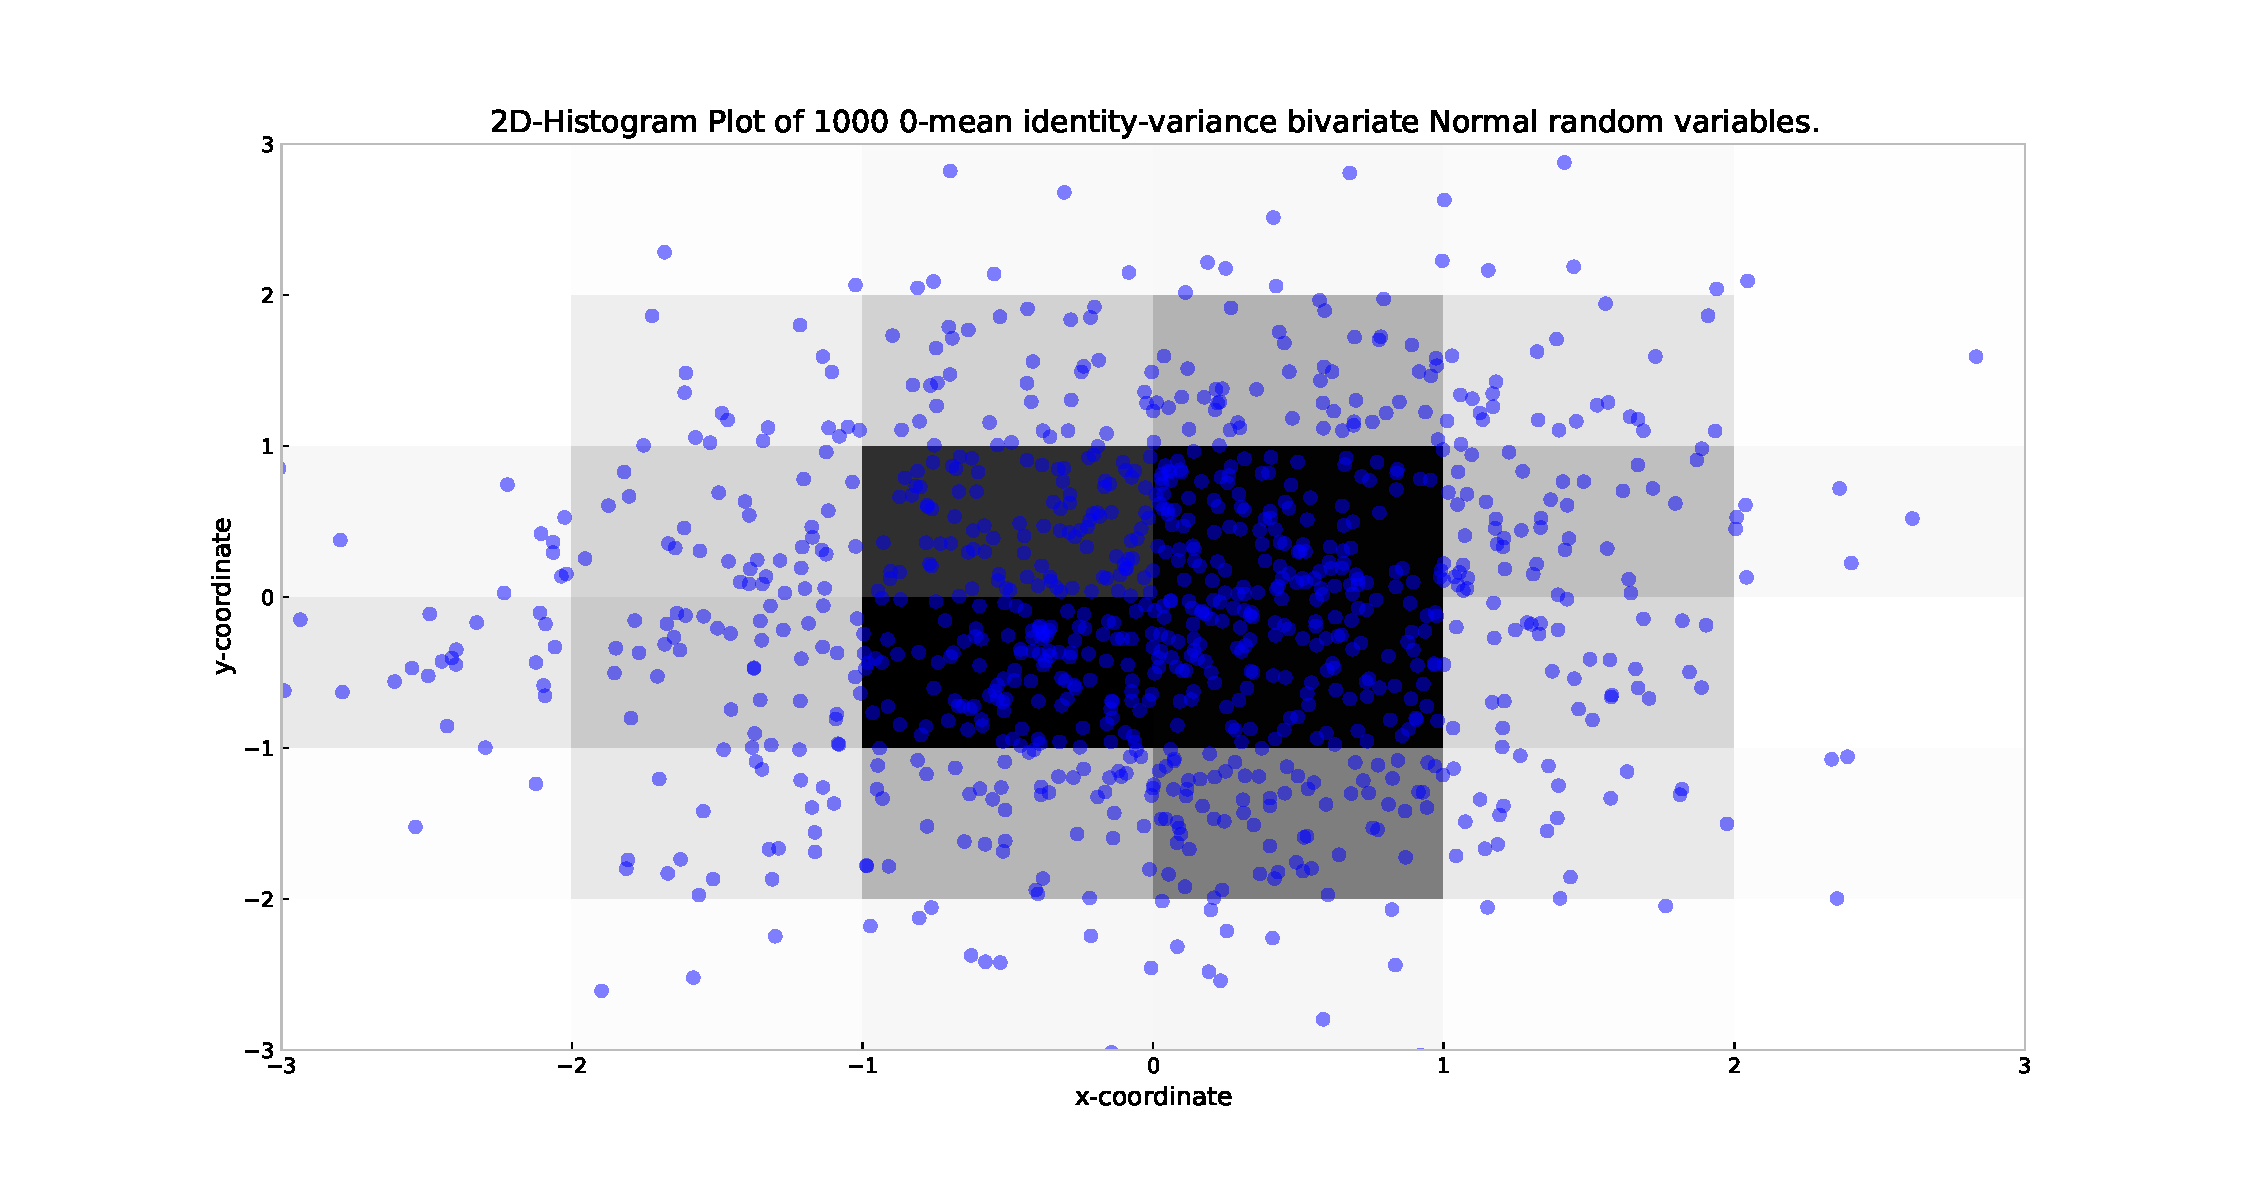
\includegraphics[height=10cm, width=15cm]{2d_pixel.pdf}
	\centering
	\caption{Plot for toy example of pixellated bivariate Normal estimation.}
	\label{fig:2d_pixels}
\end{figure}\\\noindent
Figure \ref{fig:2d_pixels} demonstrates the idea behind this, showing 1000 observations of a bivariate Normal random variable with $\mathbf{\mu} = (0, 0)$ and $\Sigma = I_2$. In a traditional setting we would expect to be able to perform inference using the truly continuous raw observations. However, in this setting we are looking to infer $\mu$  and the diagonal elements of $\Sigma$ using only the bin counts, in this example with $\Delta_x = \Delta_y = 1$. 
\section{Stochastic Processes}
Another area where the literature mostly assumes we have access to truly continuous data is stochastic processes, particularly temporal stochastic processes. Some work has been done on deriving methods and results for estimating parameters for Hawkes processes where the timestamps we have access to have been placed into bins, for example in \cite{shlomovich2020monte}. We will explore how aggregation affects the resolution of inference for stochastic process, specifically in the case of Poisson processes. \\\\
Giving a classic example as treated in \cite{erlang}, imagine we are looking to estimate the number of incoming telephone calls to a telephone trunking system. If we were trying to fit parameters for a given Poisson process rate function to this, we often assume that we have access to the raw, continuous timestamps of calls made. In reality, however, we may only have access to rounded timestamps, or how many calls were made in given intervals over a day (for example, how many calls were made each hour).

In this situation, an important consideration when performing inference is: to what degree of precision do we need to record an event's timestamp (in this case, when a call was made)? Is minute-wise precision granular enough, or do we need to record timestamps with a greater degree of precision? We will see that this is dependent on the functional form of the process, as well as how intense the process itself is. As these processes often have a temporal aspect, the binning we will be doing here is time-wise.
In Figure \ref{fig:nhpp_periodic} we can see a demonstration of this. We are looking to perform inference for the parameter $\omega$ on an inhomogeneous Poisson process with  rate function of the form:
\begin{equation*}
	\lambda(t; \omega) = 1 + \cos(\omega t).
\end{equation*}
\begin{figure}[!h]
	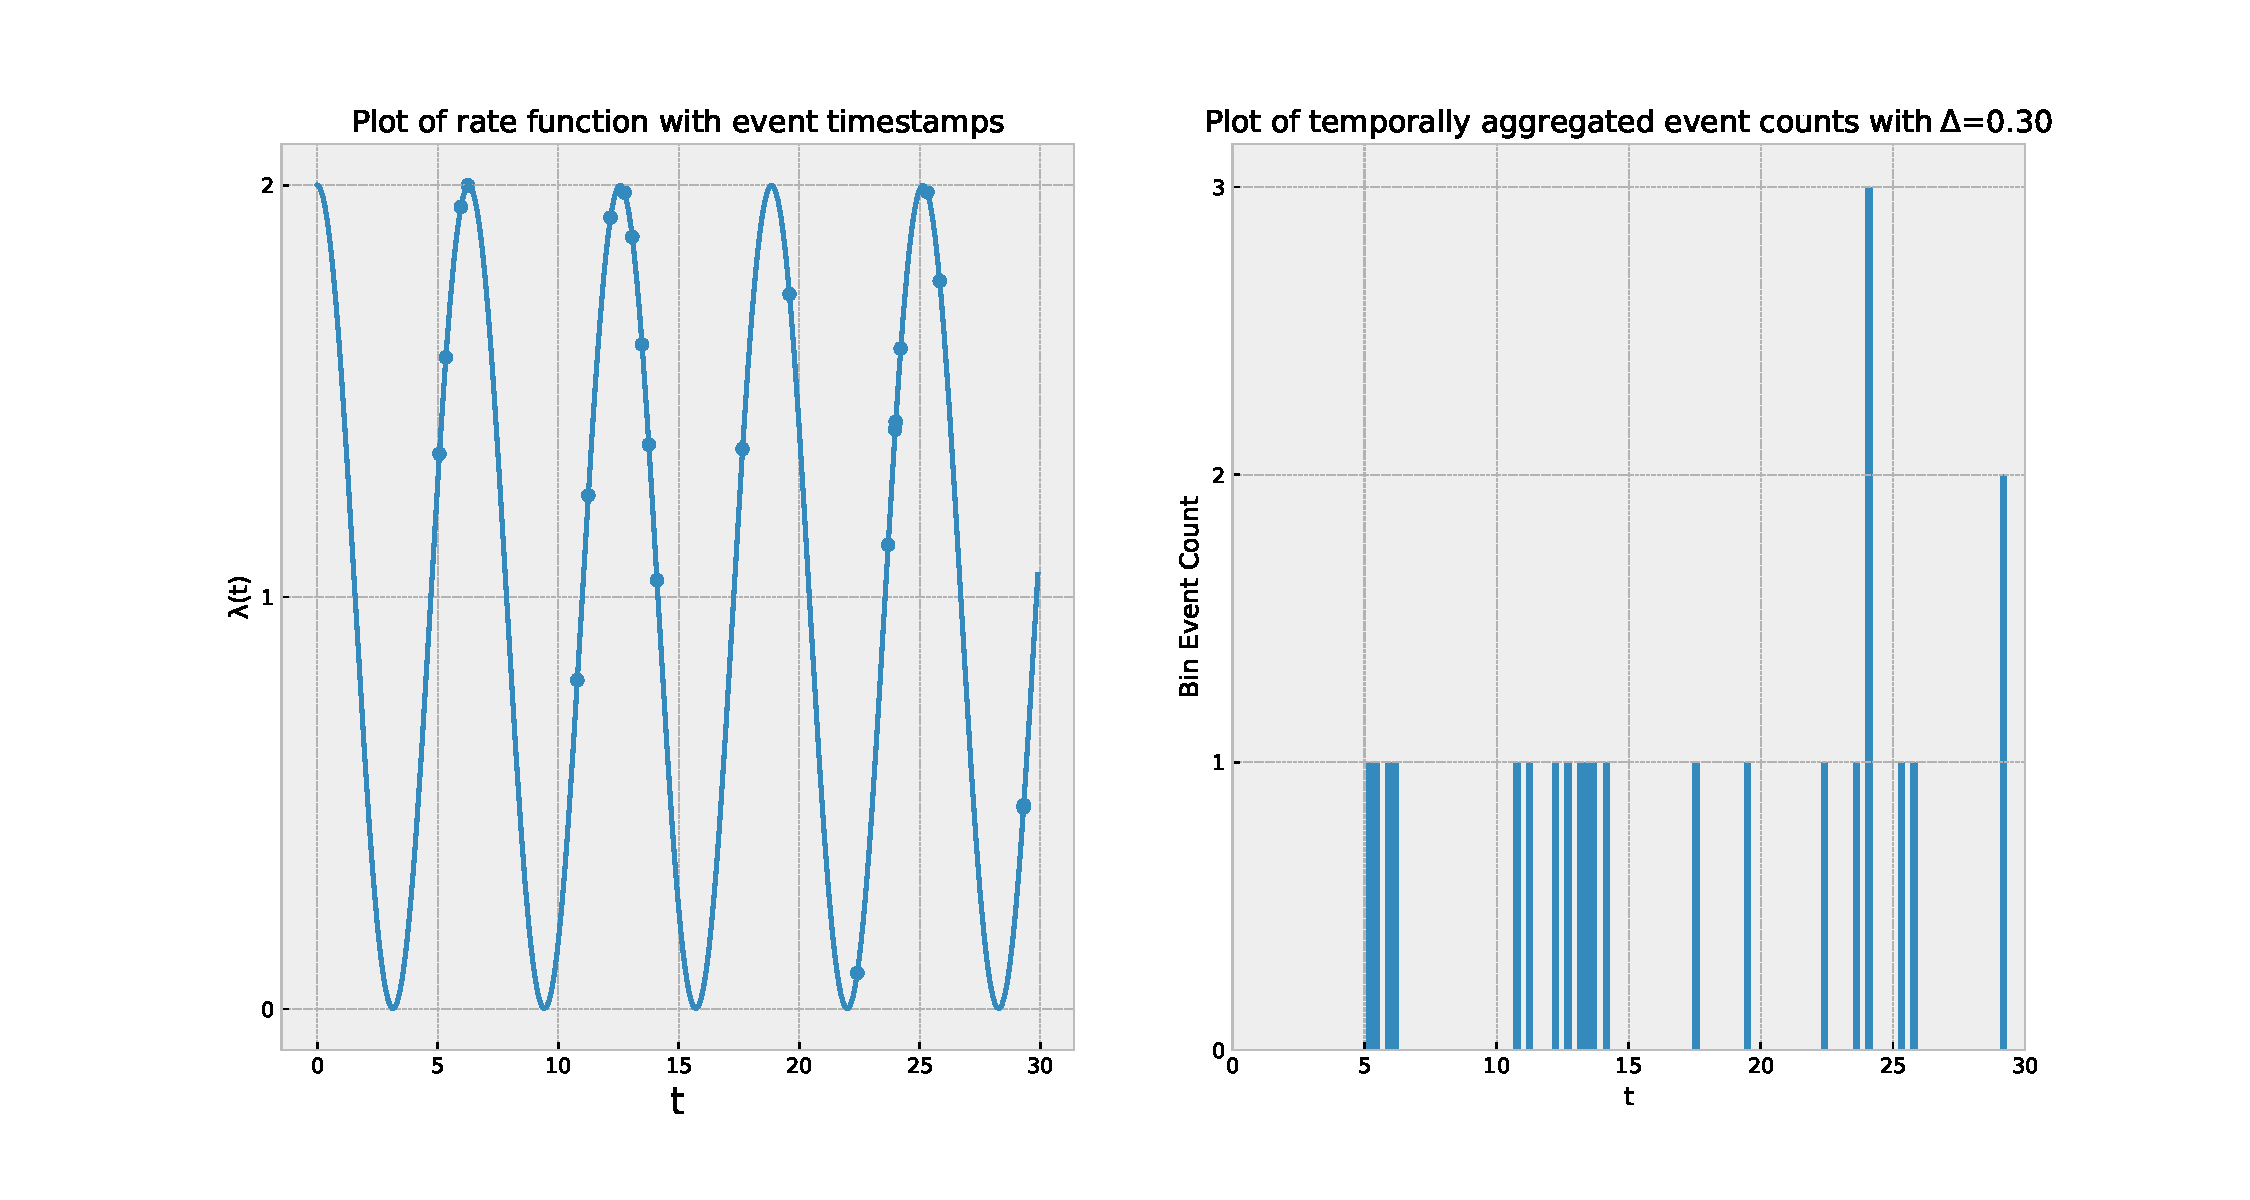
\includegraphics[height=10cm, width=15cm]{nhpp_periodic.pdf}
	\centering
	\caption{Plots for inhomogeneous Poisson process with $\lambda(t)= 1 + \cos(t)$.}
	\label{fig:nhpp_periodic}
\end{figure}\\\noindent
Again, traditionally we would expect to have access to the raw, infinitely continuous timestamps. However, in this setting we have temporal bins with $\Delta=0.4$, and we wish to use these aggregated counts to estimate the value of $\omega$ (along with providing a degree of uncertainty in our estimate). We will also explore the issue of identifiability, as over-aggregation can make it impossible to perform inference on processes whose rate functions involve periodic parameters, no matter the number of observations.

\chapter{Likelihood Theory and Identifiability}

\section{Basic Definitions}
Definitions and results in this section are from \cite{fisher_1922} and \cite{young_smith_2005}. Given independent and identically distributed observed data $x_1, \dots, x_n$ generated by a random variable $X$ from some parametric distribution with density or mass function $f_X(x; \theta)$, where $\theta = (\theta_1, ..., \theta_d)$ may be multidimensional, we say the likelihood function is defined as
\begin{equation}\label{eq:likelihood}
	L(\theta) \equiv L(\theta; x_1, ..., x_n) = f(x_1; \theta) \dots f(x_n; \theta) = \prod_{i=1}^n f(x_i; \theta).
\end{equation}
In practice, we often work instead with the log-likelihood function
\begin{equation}\label{eq:log_likelihood}
	\ell(\theta) \equiv \ell(\theta; x_1, \dots, x_n) = \log L(\theta; x_1, \dots, x_n).
\end{equation}
In cases where $\ell(\theta)$ is differentiable, we can define the score function as
\begin{equation}\label{eq:score}
	s(\theta) \equiv s(\theta; x_1, \dots, x_n) = \nabla_\theta \ell(\theta),
\end{equation}
where
\begin{equation*}
	\begin{aligned}
		\nabla_\theta = 
		\begin{pmatrix}
			\frac{\partial}{\partial \theta_1}\\[1ex]
			\vdots\\[1ex]
			\frac{\partial}{\partial \theta_d}\\
		\end{pmatrix}.
	\end{aligned}
\end{equation*}
We can use this to find the maximum likelihood estimate $\hat{\theta}$, by solving the likelihood equation (assuming certain regularity conditions hold), given by
\begin{equation*}
	s(\theta) = 0.
\end{equation*}
Finally, we can take the second derivative of the log-likelihood function to obtain the Hessian matrix, defined as
\begin{equation}
	\begin{aligned}
	\mathbf{H} &= \nabla_\theta \nabla_\theta^T \ell(\theta) \\
	&= \begin{pmatrix}
		\frac{\partial^2}{\partial \theta_1^2} & \frac{\partial^2}{\partial \theta_1 \partial \theta_2} & \dots & \frac{\partial^2}{\partial \theta_1 \partial \theta_d}\\
		\frac{\partial^2}{\partial \theta_2 \partial \theta_1} & \frac{\partial^2}{\partial \theta_2^2} & \dots & \frac{\partial^2}{\partial \theta_2 \partial \theta_d}\\
		\vdots & \vdots & \ddots & \vdots\\
		\frac{\partial^2}{\partial \theta_d \partial \theta_1} & \frac{\partial^2}{\partial \theta_d \partial \theta_2} & \dots & \frac{\partial^2}{\partial \theta_d^2}\\
	\end{pmatrix}\ell(\theta).
	\end{aligned}
\end{equation}
If we take the negative expectation (again, assuming regularity conditions hold) of this, we obtain the Fisher Information matrix as below:
\begin{equation}\label{eq:fisher}
	\mathcal{I}(\theta) = -\mathbb{E}\left[ \mathbf{H} \right].
\end{equation}

\section{The Cram\'er-Rao Lower Bound}\label{sec:crlb}
Say we have any unbiased estimator (meaning $\mathbb{E}[\hat{\theta}] = \theta$), $\hat{\theta} \equiv g(X) = g(X_1, \dots, X_n)$, of $\theta$. Then the Cram\'er-Rao Lower Bound (see e.g. \cite{rao_crlb}) states that
\begin{equation}\label{eq:crlb_unbiased}
	\text{Var}(\hat{\theta}) \geq \mathcal{I}^{-1}(\theta).
\end{equation}
This lower bound is therefore key to the results derived in this thesis. It shows that our ability to perform inference on a parameter of interest, $\theta$, is directly linked to the inverse of the Fisher Information matrix.
If we are able to quantify the loss in Fisher information as we increase the level of aggregation, we can calculate how much wider confidence intervals will be for inference performed on aggregated observations versus inference performed on raw, truly continuous, observations.

\section{Asymptotics of the MLE}\label{sec:asymptotics}
Another important consideration is how the maximum likelihood estimate is distributed for larger sample sizes. Due to the Central Limit Theorem, we can say the following about the MLE. \\
As $n \to \infty$, the maximum likelihood estimate $\hat{\theta}$ for $\theta$ is approximately Normally distributed. Again, in the multivariate setting with true parameter $\theta = (\theta_0, \dots, \theta_d)$ \cite{young_smith_2005}, what this means is that
\begin{equation*}
	\sqrt{n}(\hat{\theta} - \theta) \xrightarrow{d} \mathcal{N}\left(\mathbf{0}, \mathcal{I}^{-1}(\theta) \right).
\end{equation*}
Put simply, for sufficiently large $n$, $\hat{\theta}$ follows a multivariate Normal distribution with mean vector of $\theta$, and covariance matrix $\Sigma = \mathcal{I}^{-1}(\theta)/n$. \\
This will allow us to directly compare our estimates in aggregated settings versus in raw, truly continuous settings.

\section{Identifiability}\label{sec:identifiability}
An important property which we will refer to in Section \ref{sec:trig_rate} is identifiability. Identifiability is a statistical property which is required to be satisfied in order for us to be able to identify parameters for a model, given data.

Given a parametric distribution, with associated parameter space $\Theta$, model identifiability occurs if there exists a unique bijective mapping from $\Theta$ to the model space, $\mathcal{H} = \{ H_\theta: \theta \in \Theta \}$ \cite{rothenburg_1971}. In a practical sense, this can be thought of in terms of the log-likelihood function. So, given some data $x_1,\dots,x_n$, and log-likelihood function $\ell(\theta; x_1, \dots, x_n)$, then the model is identifiable if, for any $\theta, \phi \in \Theta$,
\begin{equation*}
	\ell(\theta; x_1, \dots, x_n) = \ell(\phi; x_1, \dots, x_n) \implies \theta = \phi.
\end{equation*}
When we discuss identifiability, typically it is implied to mean global identifiability as defined above, where a model is globally identifiable if the maximum likelihood estimate is unique. However, this is usually very difficult to verify, and so often studies focus on a weaker form instead: local identifiability.
A parameter $\theta$ is said to be locally identifiable if there exists a neighbourhood around $\theta$ such that there exists no $\phi \neq \theta$ such that $\ell(\theta; x_1,\dots,x_n) = \ell(\phi; x_1,\dots,x_n)$. \\\\
An important result in this area is that the Fisher Information matrix is non-singular if and only if $\theta$ is locally identifiable \cite{rothenburg_1971}. In the single-parameter setting, practically this means that the model is locally identifiable if and only if the second-derivative of the log-likelihood function is non-zero (as this would be the only value that makes the Fisher Information matrix singular).


\chapter{Probability Distributions}

We begin by investigating the effect of aggregation on our ability to perform inference for univariate and bivariate probability distributions.

\section{Poisson Distribution}

The first distribution we will look at is the Poisson, a discrete distribution. We say that a random variable $X$ follows a Poisson$(\lambda)$ distribution if it has probability mass function
\begin{equation*}
	f_X(x ; \lambda) = \frac{\lambda^x e^{-\lambda}}{x!}, \quad \quad x \in \mathbb{N}_0, \lambda > 0.
\end{equation*}

\subsection{Raw Observations}
Now, say we observe the raw, unaggregated values for $n$ i.i.d observations $x_1, \dots, x_n$ where $x_1 \sim$ Poisson$(\lambda)$. We have likelihood and log-likelihood functions given by
\begin{equation*}
	\begin{aligned}
		L(\lambda; x_1, \dots, x_n) &= \prod_{i=1}^n \frac{\lambda^{x_i} e^{-\lambda}}{x_i!} , \\
		\ell(\lambda ; x_1, \dots, x_n) &= \log(\lambda) \sum_{i=1}^n{x_i} - n \lambda - \sum_{i=1}^n{\log(x_i)}.
	\end{aligned}
\end{equation*}
Taking first and second derivatives of the log-likelihood with respect to $\lambda$, we obtain:
\begin{equation*}
	\begin{aligned}
		\frac{\partial l}{\partial \lambda} &= \frac{\sum_{i=1}^n{x_i}}{\lambda} - n \\
		\frac{\partial^2 l}{\partial \lambda^2} &= -\frac{\sum_{i=1}^n{x_i}}{\lambda^2}.
	\end{aligned}
\end{equation*}
If we then set the first derivative equal to 0, we obtain the MLE $\hat{\lambda} = \sum{x_i}/n = \bar{x}$. We can also use the second derivative to calculate the Fisher information as follows:

\begin{equation*}
	\begin{aligned}
		\mathcal{I}(\lambda) &= -\mathbb{E}\left(\frac{\partial^2 l}{\partial \lambda^2} \right) \\
		&= \frac{1}{\lambda^2}\mathbb{E} \left(\sum_{i=1}^n x_i \right) = \frac{n \lambda}{\lambda^2} \\
		&= \frac{n}{\lambda}.
	\end{aligned}
\end{equation*}

\subsection{Aggregated Observations}

If, instead of seeing the true values, we can only observe how many values we have in each $\Delta$-sized bin, we will derive a different likelihood and log-likelihood function. For $\Delta=2$, we have:
\begin{equation*}
	B_0 = \{0, 1\}, B_1 = \{2, 3 \}, \dots, B_k = \{ 2k, 2k+1 \},
\end{equation*}
with associated $n_k = \#\{x_i: x_i \in B_k\}$, resulting in the probability of being in $B_k$ as follows:
\begin{equation}\label{eq:pois_bin_prob}
	\begin{aligned}
		\mathbb{P}(x \in B_k; \lambda) &= \frac{\lambda^{2k}e^{- \lambda}}{(2k)!} + \frac{\lambda^{2k+1}e^{-\lambda}}{(2k+1)!} \\
		&= \frac{e^{-\lambda}\lambda^{2k}}{(2k)!} \left( 1+ \frac{\lambda}{2k+1} \right).
	\end{aligned}
\end{equation}
This results in our $\Delta=2$ likelihood and log-likelihood functions being of the form:
\begin{equation*}
	\begin{aligned}
	L(\lambda; n_0, n_1, \dots) &= \prod_{k=0}^\infty \left(\frac{e^{-\lambda}\lambda^{2k}}{(2k)!} \left( 1+ \frac{\lambda}{2k+1} \right) \right)^{n_k},\\
	\ell(\lambda; n_0, n_1, \dots) &= \sum_{k=0}^\infty n_k \left( 2k \log\lambda - \lambda - \log((2k)!) + \log \left(1 + \frac{\lambda}{2k+1} \right)\right).
	\end{aligned}
\end{equation*}
Again, taking derivatives of our log-likelihood function with respect to $\lambda$, we obtain:
\begin{equation*}
	\begin{aligned}
		\frac{\partial l}{\partial \lambda} &= \sum_{k=0}^\infty n_k \left(\frac{2k}{\lambda} - 1 + \frac{1}{2k + \lambda + 1} \right) \\
		\frac{\partial^2 l}{\partial \lambda^2} &= - \sum_{k=0}^\infty n_k \left( \frac{2k}{\lambda^2} + \frac{1}{(2k + \lambda + 1)^2} \right).
	\end{aligned}
\end{equation*}

\subsection{Information Loss}
Our aim is to see how much information is lost by aggregating the data. If we can calculate the Fisher information in the aggregated cases, we will be able to compare it with the raw case to see what the effect has been. 

There is one source of randomness in the expression for the log-likelihood's second derivative: $n_k$, the number of observations in bin $B_k$. If we look at the count in an individual bin as a random variable, we have evaluated the probability $p_k$ of an observation lying in this bin in Equation \ref{eq:pois_bin_prob}. 

Further, any individual observation either is in or is not in the bin, meaning the outcome of an individual observation for bin $B_k$ will be Bernoulli distributed. And so, for $n\geq1$ total observations, our count $n_k$ in bin $B_k$ will be Binomially distributed with $n$ total trials and $p_k$ probability of lying in bin $B_k$. The expected value for a bin count is then simply the product of these:
\begin{equation}\label{eq:binomial_bin}
	\mathbb{E}(n_k) = n p_k.
\end{equation}
We can plug in the result from Equation \ref{eq:pois_bin_prob} as our $p_k$, and so for $\Delta=2$ we have:
\begin{equation*}
	\begin{aligned}
		\mathcal{I}(\lambda) &= - \mathbb{E}\left[\frac{\partial^2 l}{\partial \lambda^2} \right] \\
		&= n\sum_{k=0}^\infty \frac{e^{-\lambda}\lambda^{2k}}{(2k)!} \left( 1+ \frac{\lambda}{2k+1} \right) \left( \frac{2k}{\lambda^2} + \frac{1}{(2k + \lambda + 1)^2} \right)
	\end{aligned}
\end{equation*}
Viewing this as a function of $\lambda$, we can see how much information will be lost for $\Delta = 2$ for different values of $\lambda$  for a Poisson distributed random variable. To do this we calculate the following `Information Loss (IL)':
\begin{equation}\label{eq:info_loss}
	IL = 1 - \frac{\mathcal{I}_{bin}(\lambda)}{\mathcal{I}_{cts}(\lambda)}.
\end{equation}
Figure \ref{fig:poisson_info_loss} shows the effect of aggregation on IL for varying values of $\lambda$.
\begin{figure}[!h]
	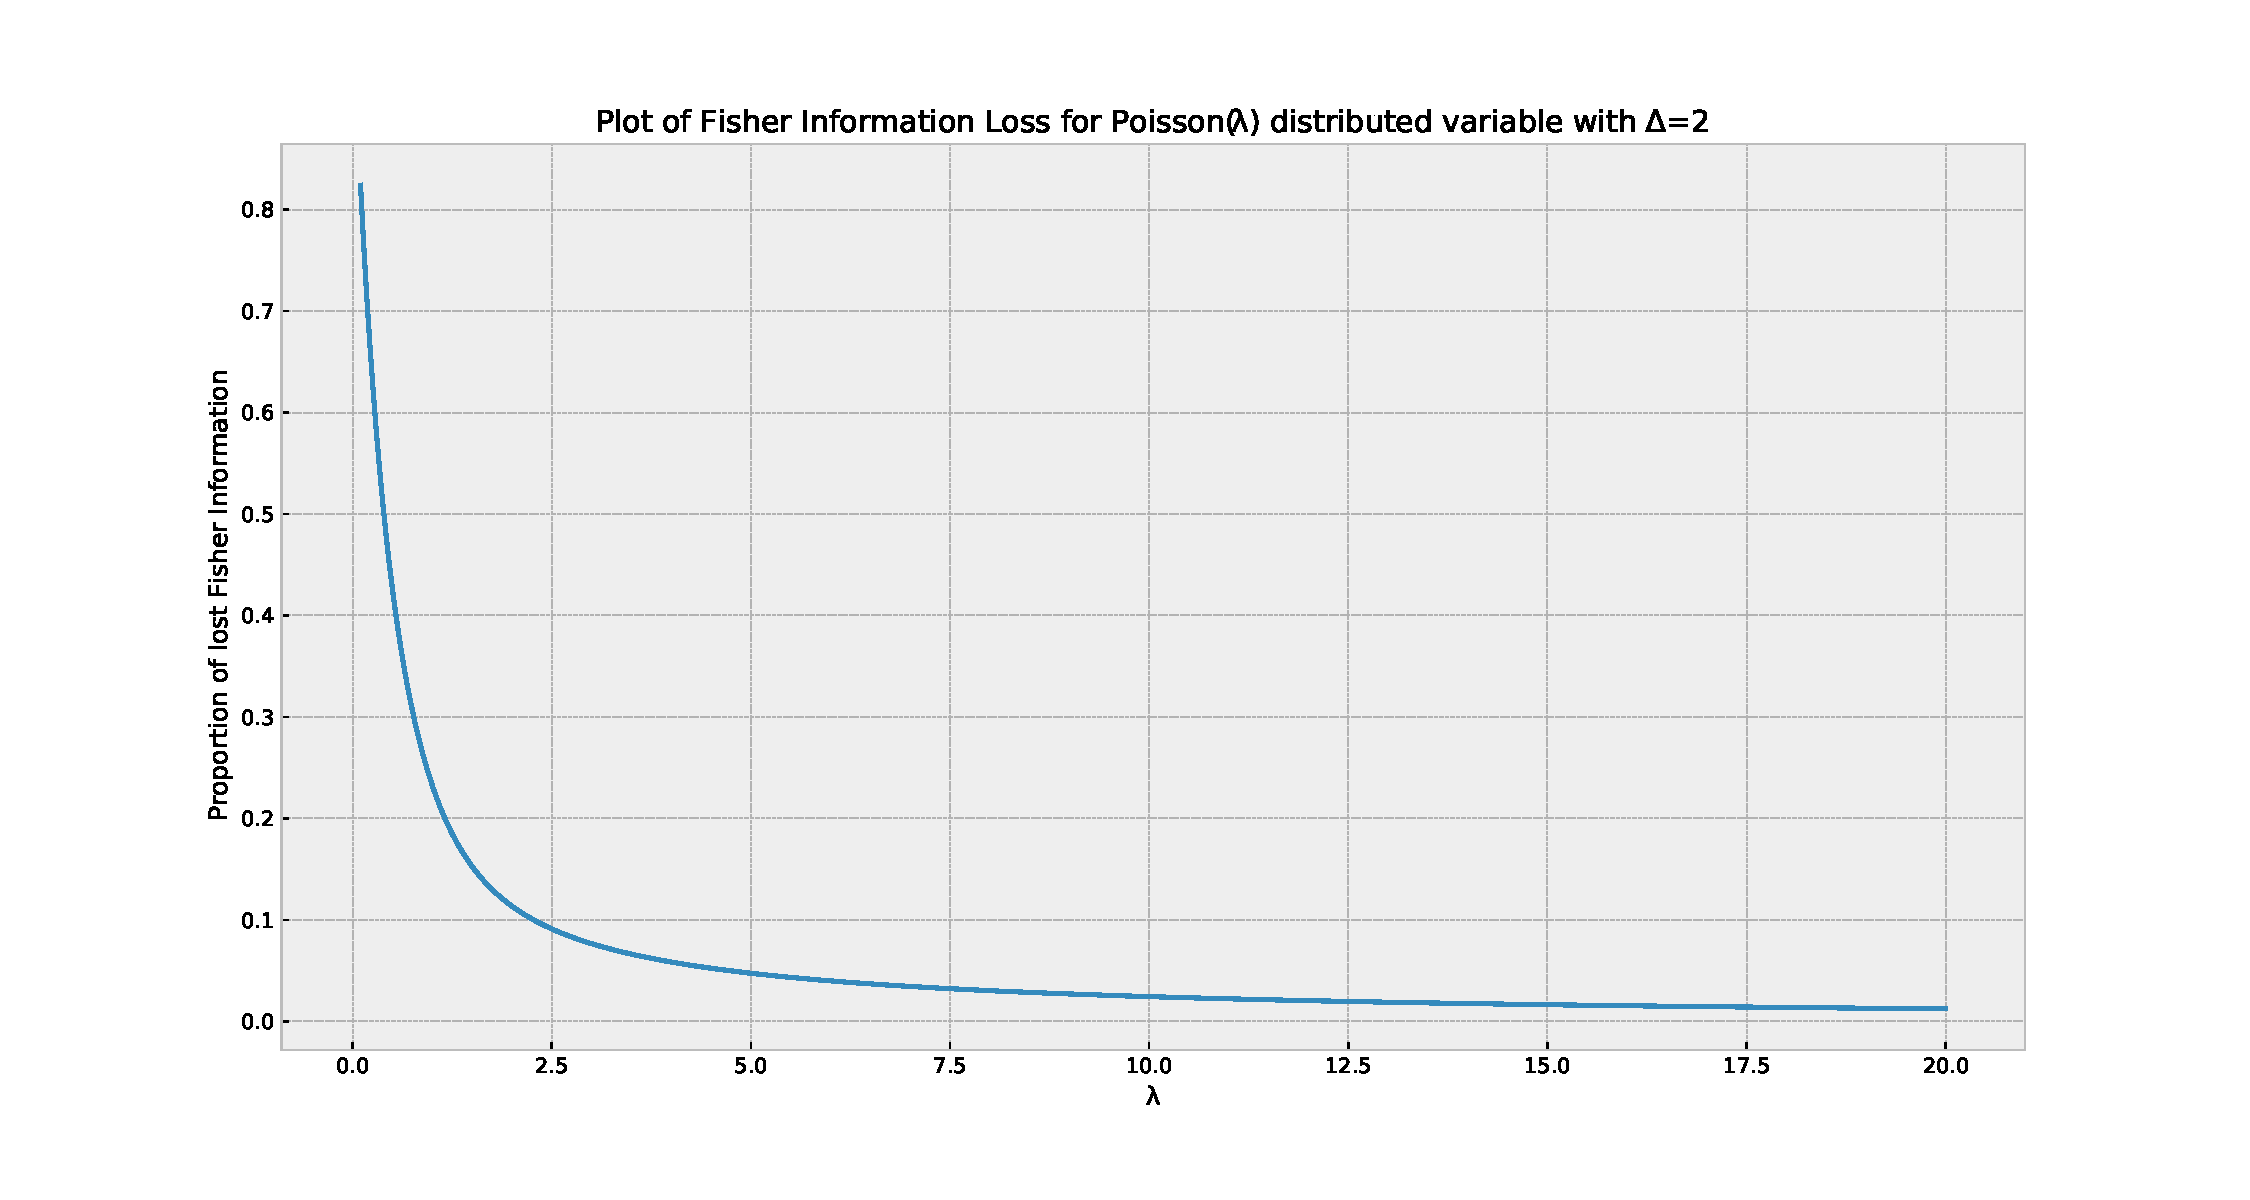
\includegraphics[height=10cm, width=14cm]{poisson_info_loss.pdf}
	\centering
	\caption{Fisher Information lost by observing $\Delta=2$ aggregated Poisson observations.}
	\label{fig:poisson_info_loss}
\end{figure}\\\noindent
This aligns well with intuition; for larger values of $\lambda$ we expect to see more varied observations as $\var(X) = \lambda$ for $X \sim$ Poisson$(\lambda)$ (and so less observations in each bin, relatively speaking). This means the aggregation will have less of an effect on our ability to perform inference relative to that performed on raw observations.

\newpage
\section{Exponential Distribution}
We now turn our attention to continuous distributions; we begin with the Exponential distribution. A random variable $X$ follows an Exponential$(\lambda)$ distribution if it has probability density function
\begin{equation*}
	f_X(x; \lambda) = \lambda e^{- \lambda x}, \quad \quad x \geq 0, \lambda > 0.
\end{equation*}
The effect of aggregation on Exponential data has been treated previously in the literature. In \cite{rounded_exp}, another approach is presented for performing inference in this setting, along with a Bayesian application. This approach involves calculating a sufficient statistic and using this to perform inference. However, this approach depends on specific properties of the Exponential distribution. For example, results in this paper rely on the sum of Exponential random variables following a Gamma distribution, along with other connections to the Geometric distribution. 

We will not be able to rely on these properties for general inference problems, such as when performing inference on Normally distributed random variables. Our aim is to provide an approach which makes fewer assumptions about the functional form of the distribution. We do this in order to make it more generally applicable. Ultimately --- other than regularity conditions holding --- the main property we require is purely that we can derive the log-likelihood function in both the continuous and aggregated cases. Here we provide an approach similar to that for the Poisson distribution (and as will be seen soon, for Normally distributed random variables also).
\subsection{Continuous Observations}
If we are able to record the truly continuous values for $n$ i.i.d observations $x_1,\dots,x_n$ where $x_1 \sim$ Exponential$(\lambda$), we obtain the log-likelihood function (and its derivatives):
\begin{equation*}
	\begin{aligned}
		\ell(\lambda; x_1,\dots, x_n) &= n \log(\lambda) - \lambda \sum_{i=1}^n x_i, \\
		\frac{\partial l}{\partial \lambda} &= \frac{n}{\lambda} - \sum_{i=1}^n x_i \\
		\frac{\partial^2 l}{\partial \lambda^2} &= -\frac{n}{\lambda^2} \\
		\implies \mathcal{I}(\lambda) &= \frac{n}{\lambda^2}.
	\end{aligned}
\end{equation*}
\subsection{Aggregated Observations}
In the case where we can only observe aggregated observations --- with observed counts $n_k$ for how many observations lie within each $\Delta$-sized bin, $B_k$ --- we have:
\begin{equation*}
	\begin{aligned}
		\mathbb{P}(x \in B_k; \lambda) &= \int_{x=k\Delta}^{(k+1)\Delta}{\lambda e^{- \lambda x} \diff x} = e^{- \lambda k\Delta}(1 - e^{- \lambda}) \\
		L(\lambda ; n_0, n_1, \dots) &= (1-e^{- \Delta\lambda})^{n_0}(e^{- \Delta\lambda} - e^{- 2\Delta\lambda})^{n_1} \dots (e^{- \lambda k\Delta} - e^{-\lambda (k+1)\Delta})^{n_k} \dots \\
		&= \prod_{k=0}^{\infty}{e^{- \lambda k \Delta n_k}(1 - e^{- \lambda \Delta})^{n_k}}, \\
		\ell(\lambda; n_0, n_1, \dots) &= \sum_{k=0}^\infty n_k \left(\log(1 - e^{- \lambda \Delta}) - \lambda k \Delta \right) \\
		\frac{\partial l}{\partial \lambda} &= \sum_{k=0}^\infty n_k \left(\frac{\Delta}{e^{\lambda \Delta} - 1} - k \Delta \right)\\
		\frac{\partial^2 l}{\partial \lambda^2} &= - \frac{\Delta^2}{(e^{\lambda \Delta} - 1)^2} \sum_{k=0}^\infty {n_k} \\
		&= - \frac{n\Delta^2}{(e^{\lambda \Delta} - 1)^2} \quad \text{($\sum n_k$ is total number of observations, $n$)}.
	\end{aligned}
\end{equation*}
We can now take the negative expected value of this to obtain the Fisher information for $\lambda$ in the binned setting:
\begin{equation}\label{eq:exp_fisher}
	\mathcal{I}_{bin}(\lambda) = - \mathbb{E}\left[ \frac{\partial^2 l}{\partial \lambda^2} \right] = \frac{n\Delta^2}{(e^{\lambda \Delta} - 1)^2}.
\end{equation}
\newpage
\subsection{Information Loss}
Similar to the Poisson case, we are interested in calculating the proportion of information that is lost, IL, by observing aggregated data instead of the raw data. Using the same approach as defined in Equation \ref{eq:info_loss}, we calculate and plot the lost information in Figure \ref{fig:exp_info_loss} below.
\begin{figure}[!h]
	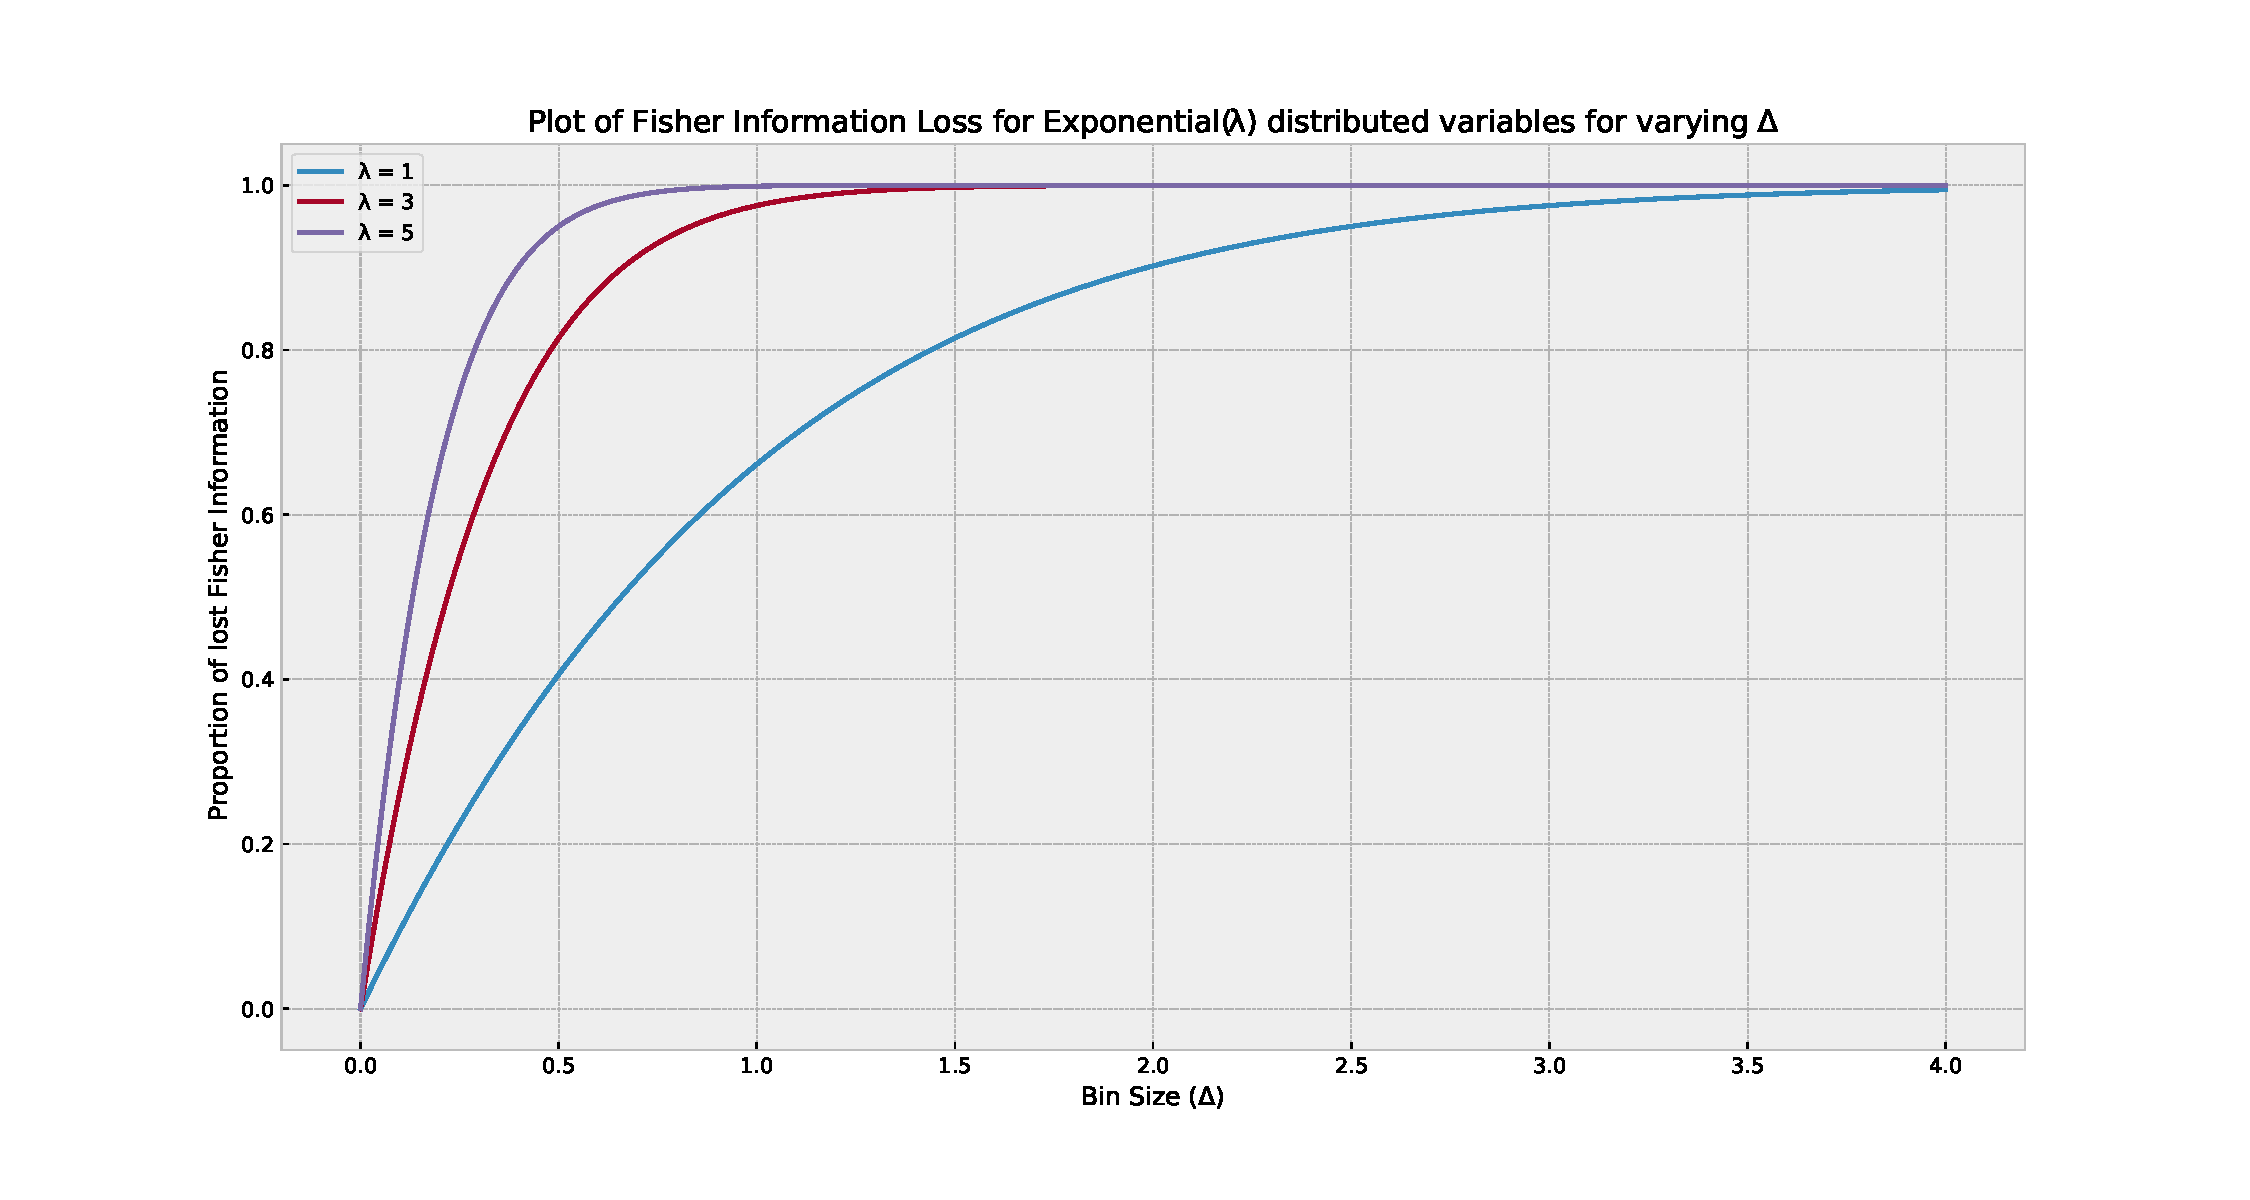
\includegraphics[height=10cm, width=14cm]{exp_info_loss.pdf}
	\centering
	\caption{Fisher Information lost by observing varying $\Delta$-aggregated Exponential observations.}
	\label{fig:exp_info_loss}
\end{figure}\\\noindent
Again, these curves have the shape we would expect. For any chosen $\lambda$ curve, as $\Delta$ increases, the proportion of lost information quickly increases to 1.

Further, if we have a random variable $X \sim $ Exponential$(\lambda)$, we have $\var(X) = 1\lambda^2$. This means that smaller values of $\lambda$ will be more highly variable, and so aggregating the data will have less of an impact, relatively speaking.

This can be seen clearly by noting that the curve for $\lambda=1$ is always lower (and so has less lost information) than the curve for $\lambda=5$.

\newpage\noindent
Another way to look at the effect aggregation has on information is by inspecting the curvature of log-likelihood curves for a given set of observations, both aggregated and raw.

A relative decrease in information between two approaches should lead to a flattening of the log-likelihood curve around the MLE, since the observed information is directly linked to the second derivative at the MLE; and the Fisher information in the raw setting is greater in magnitude than for the aggregated.
\begin{figure}[!h]
	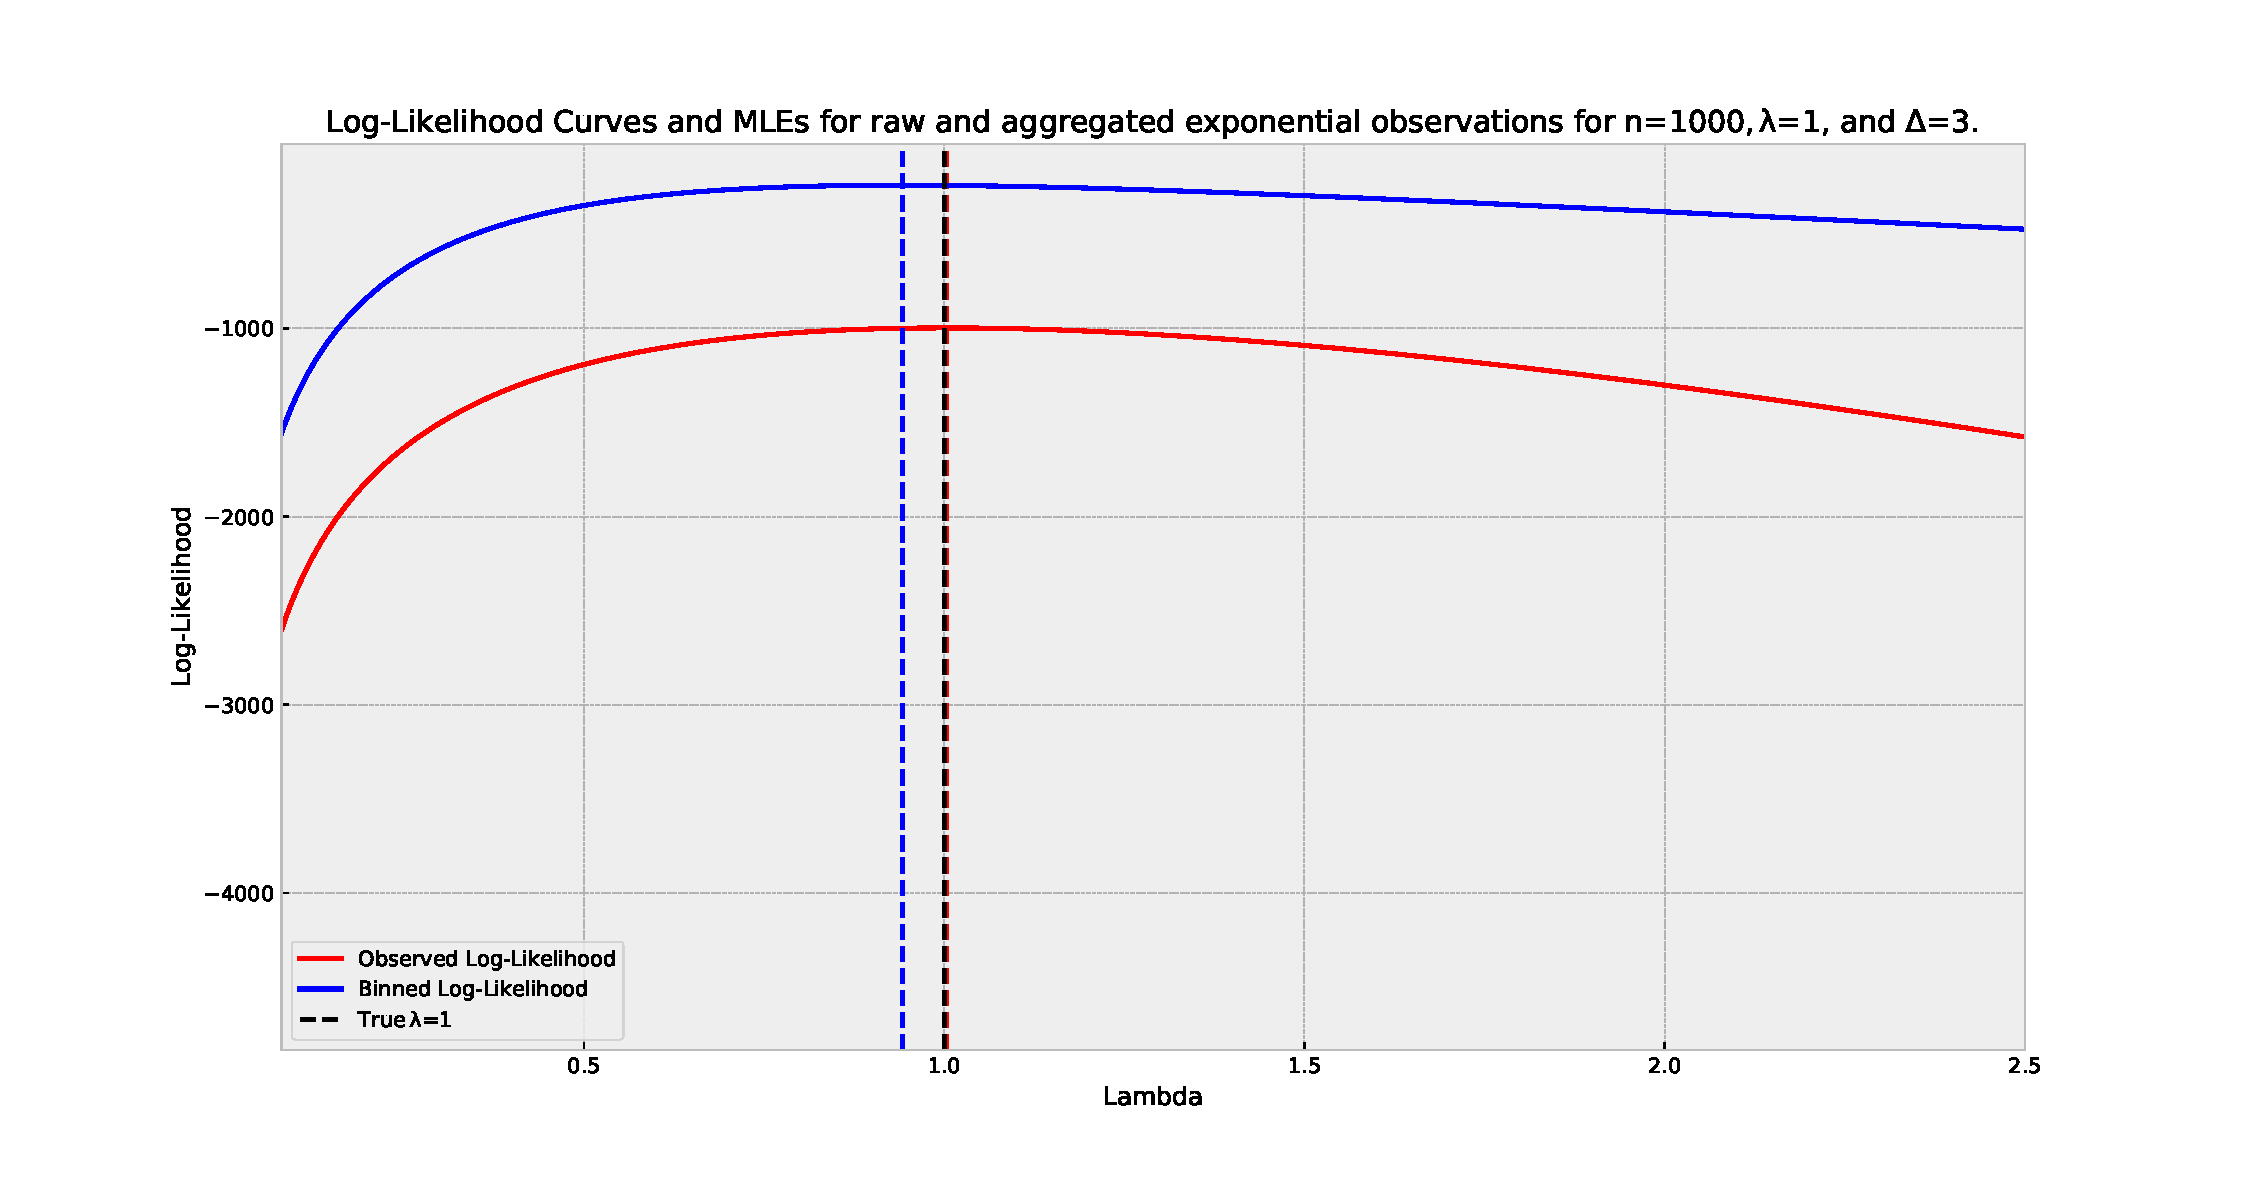
\includegraphics[height=10cm, width=14cm]{exp_log_likelihood.pdf}
	\centering
	\caption{Observed log-likelihood curves for $1000$ raw and aggregated Exponential observations.}
	\label{fig:exp_log_likelihood}
\end{figure}\\\noindent
Figure \ref{fig:exp_log_likelihood} shows the log-likelihood curves for $1000$ i.i.d. Exponential$(1)$ raw and aggregated observations, along with their MLEs represented by dotted vertical lines.

The red curve for the raw observations is clearly more curved than the blue curve for the aggregated observations. The natural interpretation of this is that values of $\lambda$ further away from the MLE $\hat{\lambda}$ are more obviously `wrong' when we have access to raw observations instead of aggregated. This is because the log-likelihood function drops away faster as we move away from the MLE. This `dropping away' is exactly what the Hessian is quantifying: the second-derivative of the log-likelihood at the MLE.

\newpage
\subsubsection{Decreasing $\Delta$ and Information Ratio}
We now calculate the Taylor expansion for the denominator in Equation \ref{eq:exp_fisher} and plug it back in. This ensures we re-obtain the continuous case Fisher information as $\Delta$ approaches 0. We have
\begin{equation*}
	\begin{aligned}
		(e^{\lambda \Delta} - 1)^2 &= \left( \lambda \Delta + \frac{(\lambda \Delta)^2}{2} + \frac{(\lambda \Delta)^3}{6} + \frac{(\lambda \Delta)^4}{24} + \dots \right)^2 \\
		&= (\lambda \Delta)^2 + (\lambda \Delta)^3 + \frac{7(\lambda \Delta)^4}{12} + \frac{(\lambda \Delta)^5}{4} + \frac{31(\lambda \Delta)^6}{360} + \frac{(\lambda \Delta)^7}{40} + \dots.
	\end{aligned}
\end{equation*}
And plugging this back into Equation \ref{eq:exp_fisher}, we obtain the following:
\begin{equation*}
	\begin{aligned}
		\mathcal{I}_{bin}(\lambda) &= \frac{n\Delta^2}{(\lambda \Delta)^2 + (\lambda \Delta)^3 + \frac{7(\lambda \Delta)^4}{12} + \frac{(\lambda \Delta)^5}{4} + \frac{31(\lambda \Delta)^6}{360} + \frac{(\lambda \Delta)^7}{40} + \dots} \\
		&= \frac{n}{\lambda^2 + \Delta \lambda^3 + \frac{7\Delta^2 \lambda^4}{12} + \frac{\Delta^3 \lambda^5}{4} + \frac{31\Delta^4 \lambda^6}{360} + \frac{\Delta^5 \lambda^7}{40} + \dots} \\
		\implies \lim_{\Delta \to 0} \mathcal{I}_{bin}(\lambda) &= \frac{n}{\lambda^2} = \mathcal{I}_{cts}(\lambda),
	\end{aligned}
\end{equation*}
thus proving that as $\Delta$ approaches 0, we re-obtain the continuous Fisher information.
\subsubsection{Asymptotics}
Another point of interest is the relationship between how slowly we can allow our number of samples, $n$, to grow relative to how fast we can allow $\Delta$ to grow without our Fisher information decreasing to 0. \\
Before we look at this relationship, we first need to define some notation. We say that a function $f(h) = \bigo(h)$ if:
\begin{equation*}
	\lim_{h \to 0} \frac{f(h)}{h} = a, \quad \text{for some finite constant } a.
\end{equation*}
Choosing some $p \in \mathbb{R}^+$, we set $\Delta:= \frac{1}{p}\log(n)$, so $\frac{n}{\Delta} \to \infty$ as $n \to \infty$, then:
\begin{equation*}
	\begin{aligned}
		\mathcal{I}(\lambda) &= \frac{\frac{1}{p^2} n \log(n)^2}{(e^{\frac{\lambda}{p} \log(n)} - 1)^2} \\
	    &= \frac{\frac{1}{p^2} n \log(n)^2}{n^{\frac{2 \lambda}{p}} - 2n^{\frac{\lambda}{p}} + 1} \\
	    &= \bigo \left( n^{1-\frac{2\lambda}{p}} (\log(n))^2 \right) \\
	    \implies \lim_{n \to \infty}\mathcal{I}(\lambda) &= 0 \text{ if } 2\lambda > p.
	\end{aligned}
\end{equation*}
From this, we see that we need to choose $p \geq 2\lambda$ to ensure the Fisher Information does not disappear to 0 as $n \to \infty$.

\newpage

\section{Normal Distribution - Univariate Case}

A random variable $X$ follows a univariate Normal$(\mu, \sigma^2)$ distribution if it has probability density function
\begin{equation}\label{eq:normal_pdf}
	f_X(x; \mu, \sigma^2) = \frac{1}{\sqrt{2 \pi \sigma^2}} \exp\left(-\frac{(x - \mu)^2}{2 \sigma^2} \right), \quad \quad x, \mu \in \mathbb{R}, \sigma > 0.
\end{equation}

\subsection{Continuous Observations}
In the case where we observe $n$ raw, continuous data points $x_1, \dots, x_n$, the log-likelihood is as follows:
\begin{equation*}
	\ell(\mu, \sigma; x_1, \dots, x_n) = -\frac{n}{2} \log(2 \pi) - \frac{n}{2} \log(\sigma^2) - \frac{1}{2 \sigma^2} \sum_{i=1}^n (x_i - \mu)^2.
\end{equation*}
We also have the Fisher Information matrix given by:
\begin{equation*}
	\mathcal{I}(\mu, \sigma) = \begin{bmatrix}
		\frac{n}{\sigma^2} & 0\\
		0 & \frac{2n}{\sigma^2}\\
	\end{bmatrix}.
\end{equation*}
\subsection{Aggregated Observations}
If instead we are only able to observe counts $n_k$ for each $\Delta$-sized bin, $B_k$, we have:
\begin{equation*}
	\begin{aligned}
		\mathbb{P}(x \in B_k) &= \Phi\left(\frac{(k+1) \Delta - \mu}{\sigma}\right) - \Phi\left(\frac{k \Delta - \mu}{\sigma}\right) \\
		L(\mu, \sigma; B_0, B_{-1}, B_1, \dots) &= \prod_{k=-\infty}^\infty \left( \Phi\left(\frac{(k + 1)\Delta - \mu}{\sigma}\right) - \Phi\left(\frac{k \Delta - \mu}{\sigma}\right) \right)^{n_k} \\
		\ell(\mu, \sigma; B_0, \dots) &= \sum_{k=-\infty}^\infty n_k \log \left(\Phi\left(\frac{(k + 1)\Delta - \mu}{\sigma}\right) - \Phi\left(\frac{k \Delta - \mu}{\sigma}\right)  \right),
	\end{aligned}
\end{equation*}
where $\Phi(\cdot)$ is the standard Normal distribution function. Now, taking derivatives, we have:
\begin{equation*}
	\begin{aligned}
		\frac{\partial \ell}{\partial \mu} &= \frac{1}{\sigma} \sum_{k=-\infty}^\infty n_k \left( 
		\frac{\phi \left( \frac{k \Delta - \mu}{\sigma} \right) - \phi \left( \frac{(k + 1) \Delta - \mu}{\sigma} \right) }
		     {\Phi \left( \frac{(k + 1) \Delta - \mu}{\sigma} \right) - \Phi \left(\frac{k \Delta - \mu}{\sigma} \right)}
		 \right) \\
		 \\
		 \frac{\partial \ell}{\partial \sigma} &= \frac{1}{\sigma^2} \sum_{k=-\infty}^\infty n_k \left( 
		\frac{(k \Delta - \mu) \phi \left( \frac{k \Delta - \mu}{\sigma} \right) - ((k + 1) \Delta - \mu)\phi \left( \frac{(k + 1) \Delta - \mu}{\sigma} \right) }
		     {\Phi \left( \frac{(k + 1) \Delta - \mu}{\sigma} \right) - \Phi \left(\frac{k \Delta - \mu}{\sigma} \right)}
		 \right),
	\end{aligned}
\end{equation*}
where $\phi(\cdot)$ is the standard Normal density function. \\\\
Now, in order to calculate the Fisher Information matrix for $\mu$ and $\sigma$, we have to take all partial second-order derivatives of our log-likelihood function, giving us the following:
\begin{equation}\label{eq:normal_d2_dmu}
	\begin{aligned}
		\frac{\partial^2 \ell}{\partial \mu^2} &= \frac{1}{\sigma^3} \sum_{k=-\infty}^\infty n_k \left( 
		\frac{((k + 1) \Delta - \mu) \phi \left( \frac{(k + 1) \Delta - \mu}{\sigma} \right) - (k \Delta - \mu) \phi \left( \frac{k \Delta - \mu}{\sigma} \right) }
		 {\Phi \left( \frac{(k + 1) \Delta - \mu}{\sigma} \right) - \Phi \left(\frac{k \Delta - \mu}{\sigma} \right)}
		 \right) \\
		 &- \frac{1}{\sigma^2} \sum_{k=-\infty}^\infty n_k \left(
		 \frac{\phi \left( \frac{(k + 1) \Delta - \mu}{\sigma} \right) - \phi \left( \frac{k \Delta - \mu}{\sigma} \right)}
		 {\Phi \left( \frac{(k + 1) \Delta - \mu}{\sigma} \right) - \Phi \left(\frac{k \Delta - \mu}{\sigma} \right)}
		 \right)^2. \\
	\end{aligned}
\end{equation}

\begin{equation}\label{eq:normal_d2_dsig}
	\begin{aligned}
		\frac{\partial^2 \ell}{\partial \sigma^2} &= \frac{1}{\sigma^5} \sum_{k=-\infty}^\infty n_k \left(
		\frac{(k \Delta - \mu)((k \Delta - \mu)^2 - 2 \sigma^2) \phi \left( \frac{k \Delta - \mu}{\sigma} \right)}
		 {\Phi \left( \frac{(k + 1) \Delta - \mu}{\sigma} \right) - \Phi \left(\frac{k \Delta - \mu}{\sigma} \right)}
		 \right) \\
		 &- \frac{1}{\sigma^5} \sum_{k=-\infty}^\infty n_k \left(
		 \frac{((m+1)d - \mu)((m+1)d - \mu)^2 - 2 \sigma^2) \phi \left( \frac{(m+1)d - \mu}{\sigma} \right)}
		 {\Phi \left( \frac{(k + 1) \Delta - \mu}{\sigma} \right) - \Phi \left(\frac{k \Delta - \mu}{\sigma} \right)}
		 \right) \\
		 &- \frac{1}{\sigma^4} \sum_{k=-\infty}^\infty n_k \left(
		 \frac{(k \Delta - \mu) \phi \left( \frac{k \Delta - \mu}{\sigma} \right) - ((k + 1) \Delta - \mu)\phi \left( \frac{(k + 1) \Delta - \mu}{\sigma} \right)}
		 {\Phi \left( \frac{(k + 1) \Delta - \mu}{\sigma} \right) - \Phi \left(\frac{k \Delta - \mu}{\sigma} \right)}
		 \right)^2.
	\end{aligned}
\end{equation}


\begin{equation}\label{eq:normal_d2_dmu_dsig}
	\begin{aligned}
		\frac{\partial^2 \ell}{\partial \mu \partial \sigma } &= \frac{1}{\sigma^4} \sum_{k=-\infty}^\infty n_k \left( 
		\frac{((k \Delta - \mu)^2 - \sigma^2) \phi \left( \frac{k \Delta - \mu}{\sigma} \right) - (((m+1)d - \mu)^2 - \sigma^2) \phi \left( \frac{(m+1)d - \mu}{\sigma} \right)}
		 {\Phi \left( \frac{(k + 1) \Delta - \mu}{\sigma} \right) - \Phi \left(\frac{k \Delta - \mu}{\sigma} \right)}
		 \right) \\
		 &- \frac{1}{\sigma^3} \sum_{k=-\infty}^\infty n_k \left(
		 \frac{\left(\phi \left( \frac{k \Delta - \mu}{\sigma} \right) - \phi \left( \frac{(k + 1) \Delta - \mu}{\sigma} \right)\right) \left( (k \Delta - \mu) \phi \left( \frac{k \Delta - \mu}{\sigma} \right) - ((k + 1) \Delta - \mu)\phi \left( \frac{(k + 1) \Delta - \mu}{\sigma} \right)\right)}
		 {\left(\Phi \left( \frac{(k + 1) \Delta - \mu}{\sigma} \right) - \Phi \left(\frac{k \Delta - \mu}{\sigma} \right)\right)^2}
		 \right).
	\end{aligned}
\end{equation}
When calculating the expected values for these derivatives, we can again use the trick employed in Equation \ref{eq:binomial_bin}:
\begin{equation*}
	\begin{aligned}
		\mathbb{E}(n_k) &= n p_k \\
		&= n \left( \Phi\left(\frac{(k+1) \Delta - \mu}{\sigma}\right) - \Phi\left(\frac{k \Delta - \mu}{\sigma}\right) \right),
	\end{aligned}
\end{equation*}
and plug this value back into equations \ref{eq:normal_d2_dmu}, \ref{eq:normal_d2_dsig}, and \ref{eq:normal_d2_dmu_dsig} to obtain:
\begin{equation}\label{eq:normal_mu_fisher}
	\begin{aligned}
		-\mathbb{E}\left[\frac{\partial^2 \ell}{\partial \mu^2}\right] &= \frac{n}{\sigma^2} \sum_{k=-\infty}^\infty 
		 \frac{\left(\phi \left( \frac{(k + 1) \Delta - \mu}{\sigma} \right) - \phi \left( \frac{k \Delta - \mu}{\sigma} \right)\right)^2}
		 {\Phi \left( \frac{(k + 1) \Delta - \mu}{\sigma} \right) - \Phi \left(\frac{k \Delta - \mu}{\sigma} \right)}
		  \\
		&- \frac{n}{\sigma^3} \sum_{k=-\infty}^\infty \left(
			((k + 1) \Delta - \mu) \phi \left( \frac{(k + 1) \Delta - \mu}{\sigma} \right) - (k \Delta - \mu) \phi \left( \frac{k \Delta - \mu}{\sigma} \right)
		\right)
	\end{aligned},
\end{equation}
\begin{equation}\label{eq:normal_sigma_fisher}
	\begin{aligned}
		-\mathbb{E}\left[\frac{\partial^2 \ell}{\partial \sigma^2}\right] &= \frac{n}{\sigma^5} \sum_{k=-\infty}^\infty  \left(
			(k \Delta - \mu)((k \Delta - \mu)^2 - 2 \sigma^2) \phi \left( \frac{k \Delta - \mu}{\sigma} \right)
		\right) \\
		&+ \frac{n}{\sigma^5} \sum_{k=-\infty}^\infty  \left(
			((m+1)d - \mu)((m+1)d - \mu)^2 - 2 \sigma^2) \phi \left( \frac{(m+1)d - \mu}{\sigma} \right)
		\right)\\
		&+ \frac{n}{\sigma^4} \sum_{k=-\infty}^\infty  \left(
			\frac{\left(
				(k \Delta - \mu) \phi \left( \frac{k \Delta - \mu}{\sigma} \right) - ((k + 1) \Delta - \mu)\phi \left( \frac{(k + 1) \Delta - \mu}{\sigma} \right)
			\right)^2}
			{\Phi \left( \frac{(k + 1) \Delta - \mu}{\sigma} \right) - \Phi \left(\frac{k \Delta - \mu}{\sigma} \right)}
		\right)
	\end{aligned},
\end{equation}
and
\begin{equation}\label{eq:normal_mu_sigma_fisher}
	\begin{aligned}
		-\mathbb{E}&\left[\frac{\partial^2 \ell}{\partial \mu \partial \sigma}\right] = -\frac{n}{\sigma^4}\sum_{k=-\infty}^\infty  \left(
			((k \Delta - \mu)^2 - \sigma^2) \phi \left( \frac{k \Delta - \mu}{\sigma} \right) - (((m+1)d - \mu)^2 - \sigma^2) \phi \left( \frac{(m+1)d - \mu}{\sigma} \right)
		\right) \\
		&+ \frac{n}{\sigma^3}\sum_{k=-\infty}^\infty  \left(
			\frac{\left(\phi \left( \frac{k \Delta - \mu}{\sigma} \right) - \phi \left( \frac{(k + 1) \Delta - \mu}{\sigma} \right)\right) \left( (k \Delta - \mu) \phi \left( \frac{k \Delta - \mu}{\sigma} \right) - ((k + 1) \Delta - \mu)\phi \left( \frac{(k + 1) \Delta - \mu}{\sigma} \right)\right)}
		 {\Phi \left( \frac{(k + 1) \Delta - \mu}{\sigma} \right) - \Phi \left(\frac{k \Delta - \mu}{\sigma} \right)}
		\right)
	\end{aligned}.
\end{equation}
By numerically evaluating Equation \ref{eq:normal_mu_sigma_fisher} for many combinations of $\mu$ and $\sigma$, we find that the sum is always equal to 0. Therefore, the off-diagonal elements in the Fisher Information matrix will also be 0. \\
This is beneficial as it shows performing inference in the aggregated setting is similar to inference performed in the continuous setting. Put simply, it means that when performing inference on both $\mu$ and $\sigma$, any errors we make in estimating $\mu$ will not affect our error in estimating $\sigma$, and vice versa. This also allows us to more simply compare losses of information for inference --- by comparing entry-wise for both $\mu$ and $\sigma$ --- rather than requiring calculation of a separate metric for the loss of information by aggregation. \\
We have the Fisher Information matrix:
\begin{equation}\label{eq:normal_binned_fisher}
	\mathcal{I}_{bin}(\mu, \sigma) = \begin{bmatrix}
		-\mathbb{E}\left[\frac{\partial^2 \ell}{\partial \mu^2}\right] & 0 \\
		0 & -\mathbb{E}\left[\frac{\partial^2 \ell}{\partial \sigma^2}\right] \\
	\end{bmatrix}.
\end{equation}
\newpage
\subsection{Information Loss}\label{subsec:normal_info_loss}
Now that we have derived the Fisher Information matrix for both continuous and aggregated observations, we are able to examine the effect of aggregation on information loss for both $\mu$ and $\sigma$.

In Figure \ref{fig:normal_0_1_info_loss}, we see the effect of increasing aggregation on performing inference on Normal$(0, 1)$ observations. The effect on $\sigma$ is typical for what we have seen in both Exponential and Poisson distributed variables: as $\Delta$ increases, the proportion of lost information quickly approaches 1. \\
\begin{figure}[!h]
	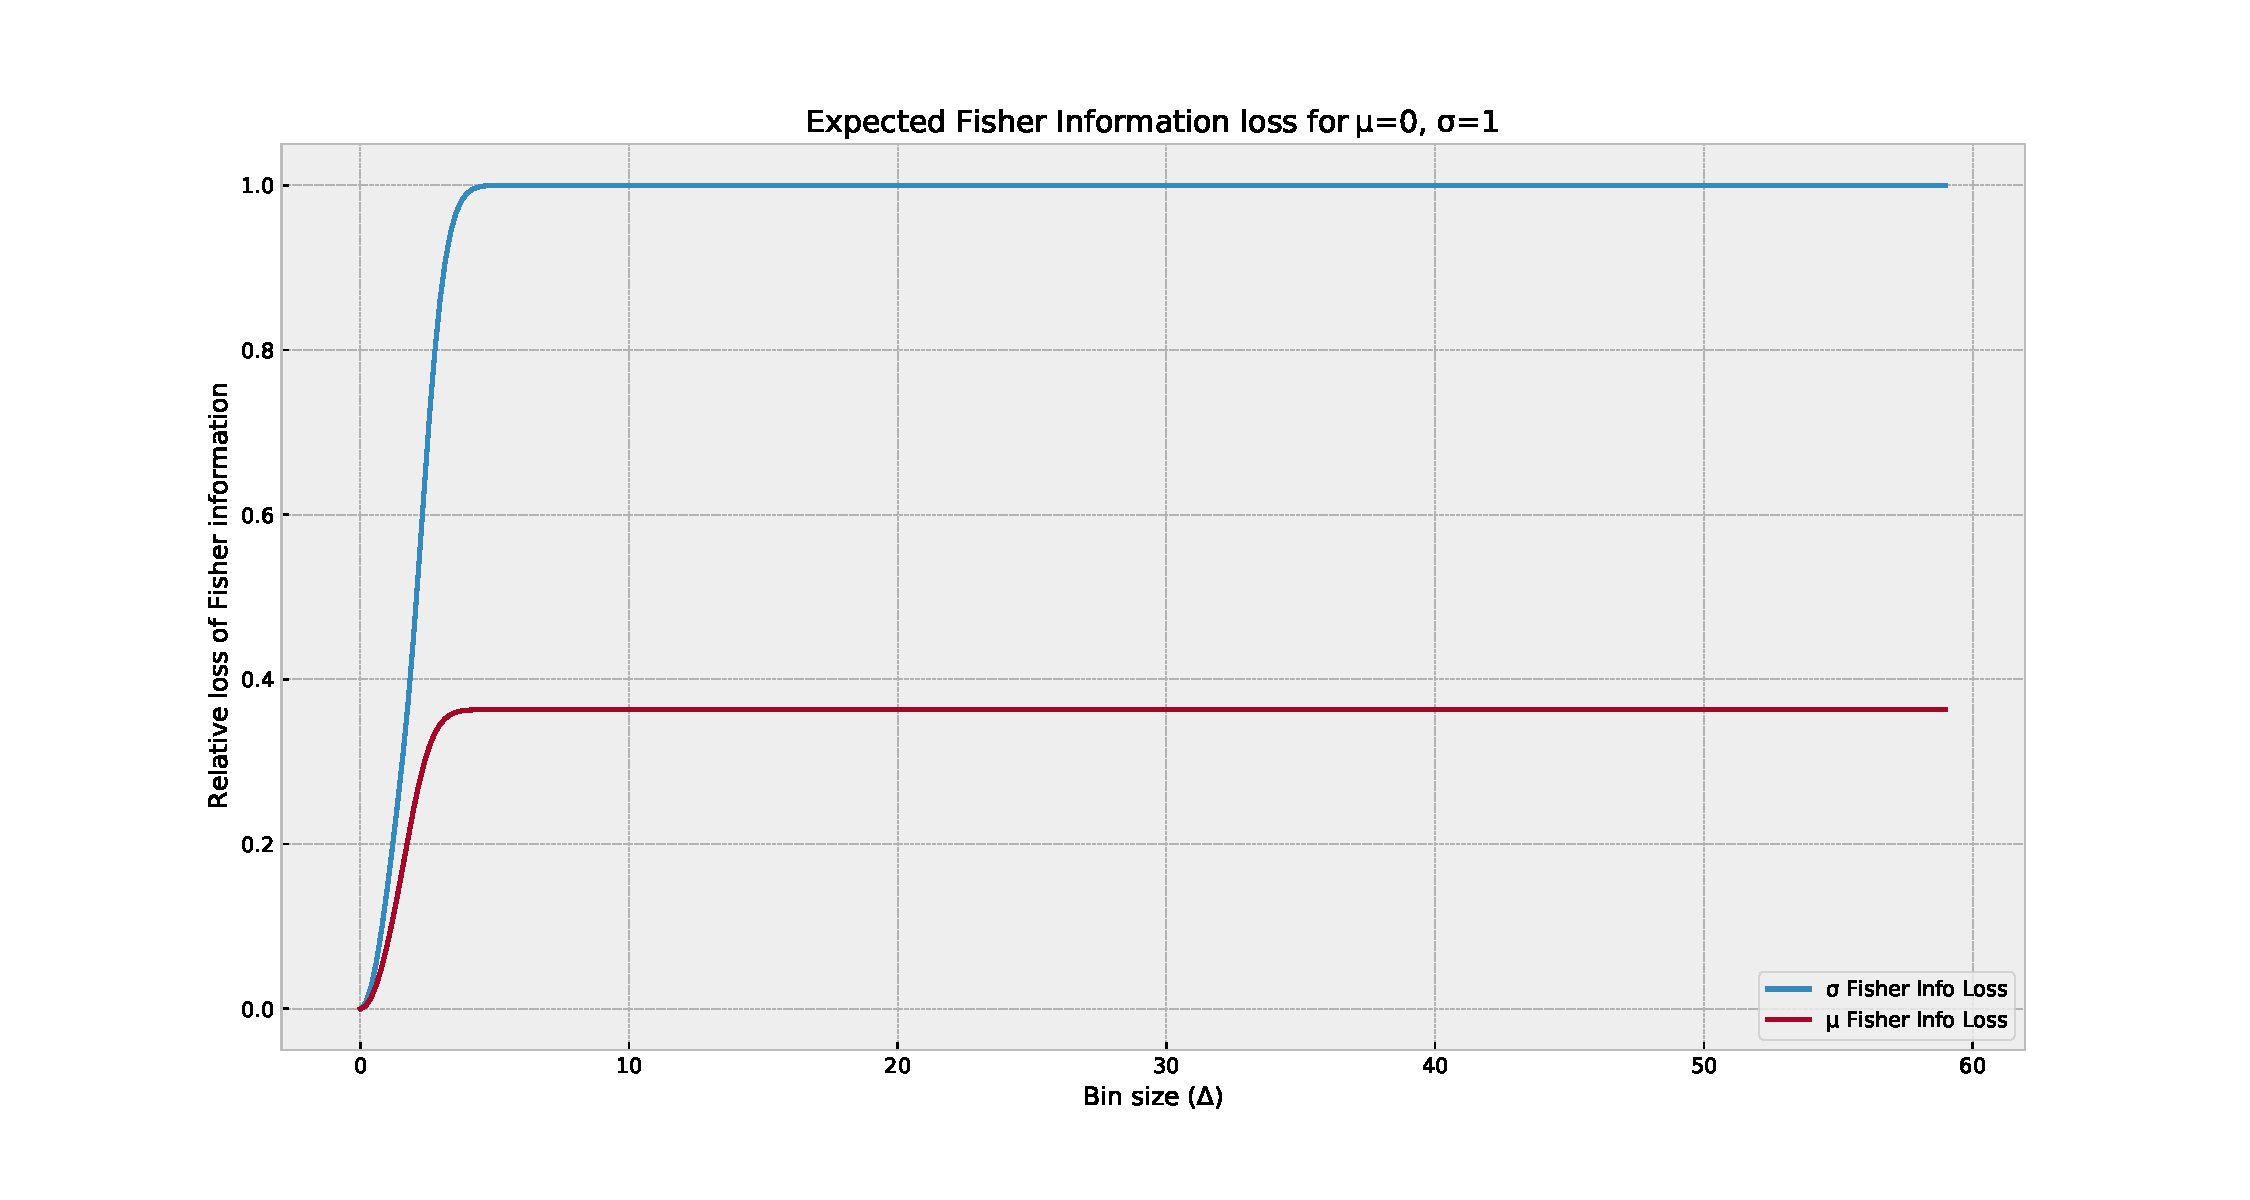
\includegraphics[height=10cm, width=14cm]{mu0sig1.pdf}
	\centering
	\caption{Fisher Information lost by observing $\Delta$-aggregated Normal(0, 1) observations.}
	\label{fig:normal_0_1_info_loss}
\end{figure}\\\noindent
However, if we look at the relative information loss for $\mu$, a different story emerges. The loss of information begins by following a similar curve, quickly shooting up with increasing $\Delta$. But when $\Delta \approx 4.5$, the curve stabilises at IL $\approx 0.36$. This is a demonstration of another effect of our bins. 

When trying to find a `location' for a location-scale distribution, in this case $\mu$, our ability to perform inference also depends on how well the edge of the bin aligns with the location parameter. If a bin edge aligns perfectly with the location parameter, our ability to perform inference does not degrade by IL approaching 1 as $\Delta$ increases. Instead, it degrades somewhat, but that degradation caps out below 1.

An intuitive way of understanding this is to imagine two infinitely large bins splitting the real line into positive and negative values, while we try to perform inference on Normal$(0, 1)$ observations. We would expect each of these bins to have approximately the same number of observations in each, as their edge is at $\mu=0$. Due to this, as more observations come in, we could still reasonably perform inference by observing the relative count in each bin. But if $\mu$ were to be significantly far away from 0, (nearly) all observations would eventually be in just one of the bins, and so our ability to perform inference would disappear. \\\\
Figure \ref{fig:normal_50_1_info_loss} demonstrates this idea further. In this situation we are performing inference on Normal(50, 1) observations. Since $\mu=50$, our bins edges do not necessarily align with the mean. This therefore means that as $\Delta$ increases, the lost information will again approach 1. However, as the bin edges move in and out of phase with $\mu$, our (relative) ability to perform inference is temporarily regained. This can be seen clearly at $\Delta$ values which divide 50, such as $\Delta=10, 25, 50$. In these instances, IL drops back to around $0.36$. \\
Another interesting development is that bin alignment has the opposite effect for performing inference on $\sigma$. Again this follows intuition: if the bins are perfectly aligned with $\mu$, we have less ability to see how variable the observations are as they will be split symmetrically about $\mu$.
\begin{figure}[!h]
	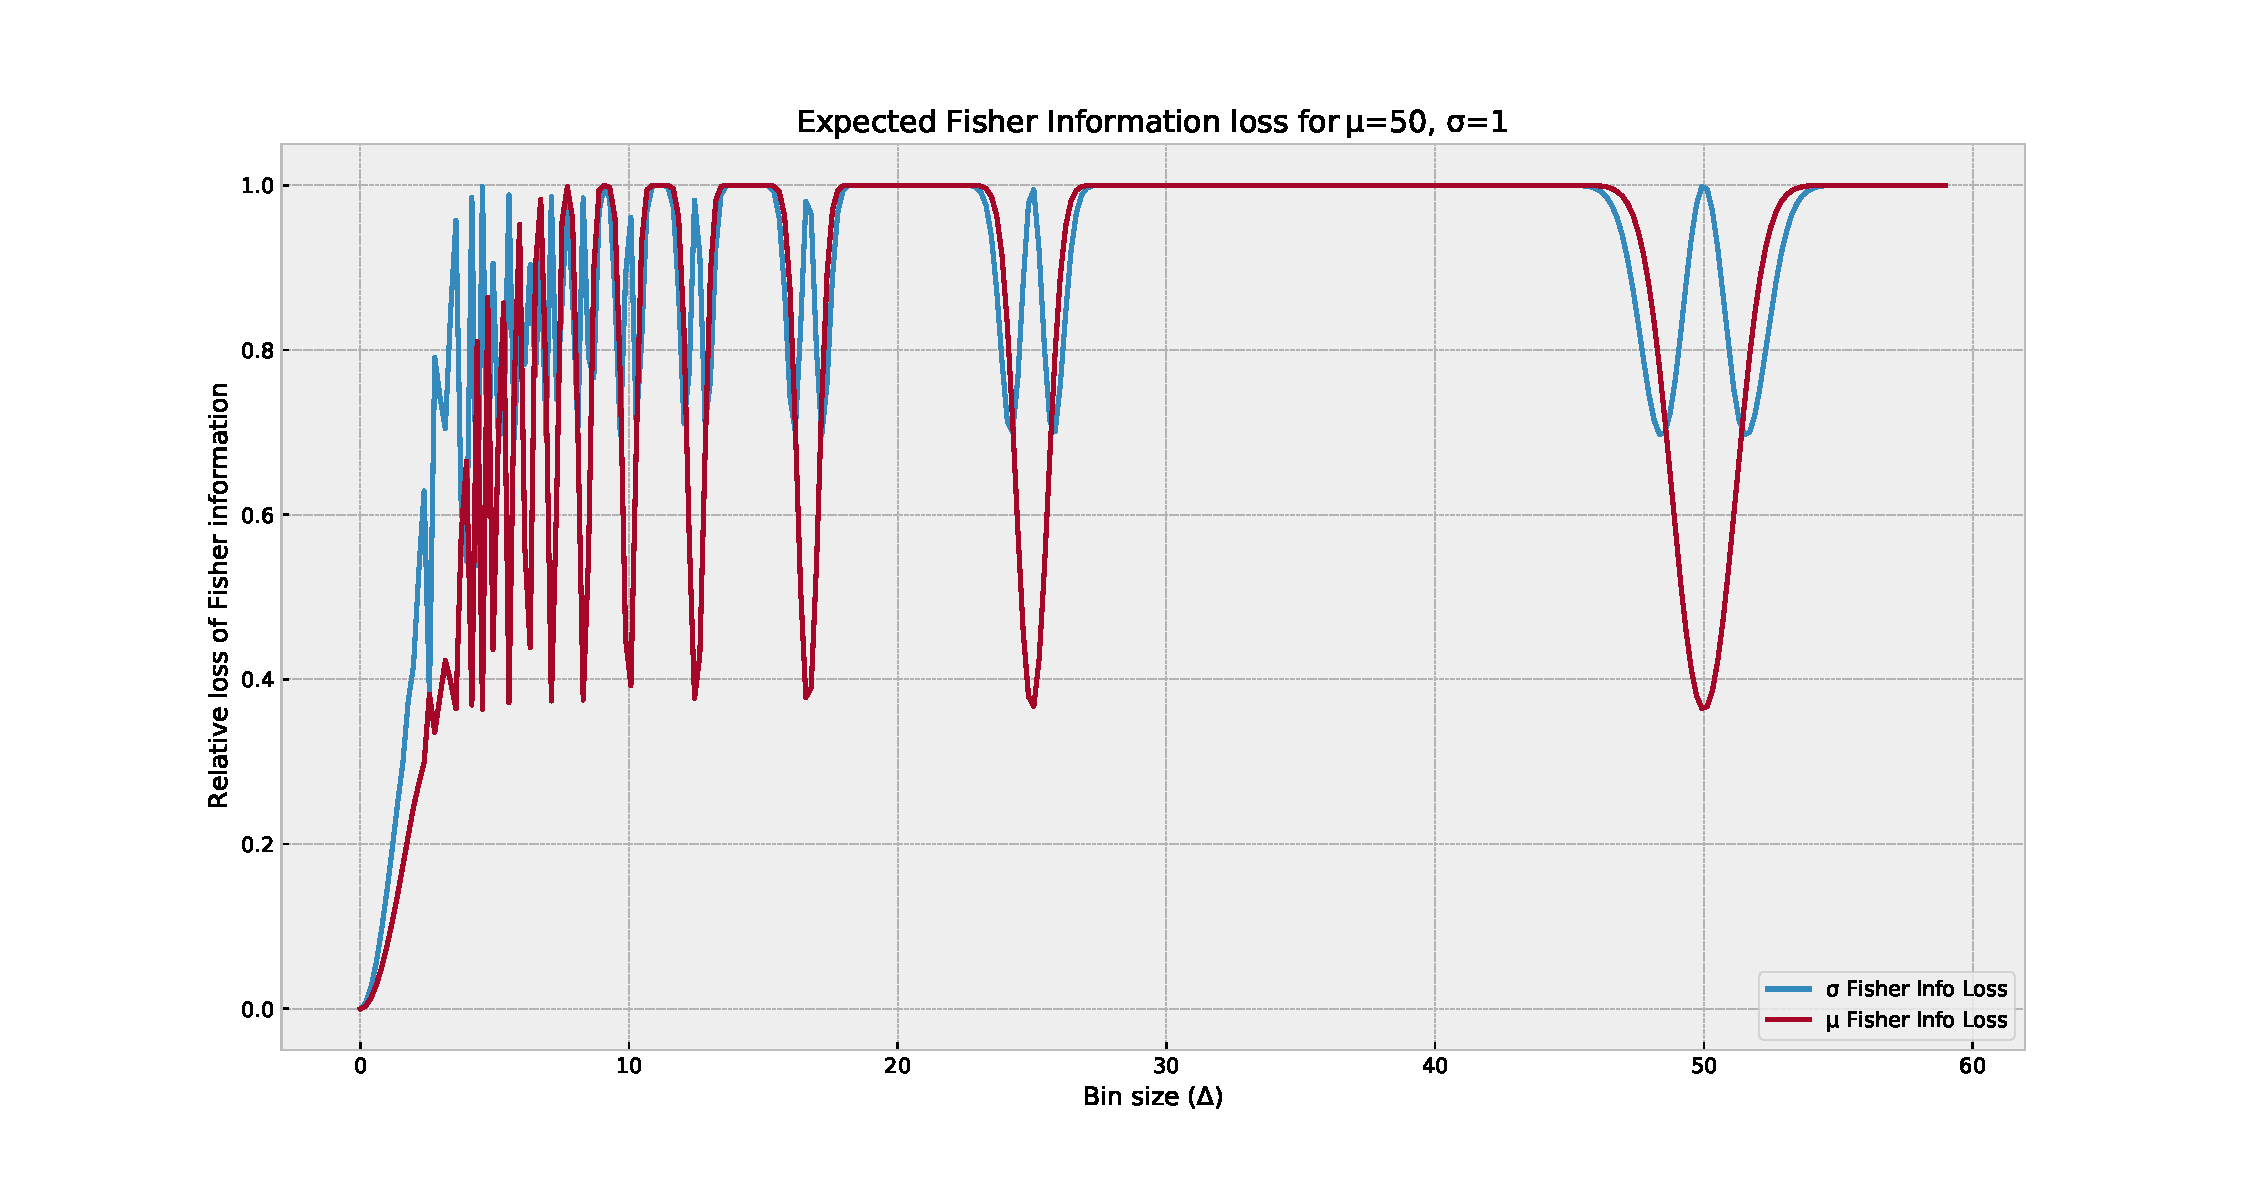
\includegraphics[height=8cm, width=14cm]{mu50sig1.pdf}
	\centering
	\caption{Fisher Information lost by observing $\Delta$-aggregated Normal(50, 1) observations.}
	\label{fig:normal_50_1_info_loss}
\end{figure}\noindent
\clearpage
\subsection{Toy Problem - Comparison with CRLB}
We finish looking at the univariate Normal distribution with a toy problem. In this problem, we have $n=500$ i.i.d samples of Normal(1, 1) random variables. We take $\sigma=1$ as known, and we are trying to perform inference on the unknown parameter, $\mu$, in the continuous case and in the aggregated case with $\Delta=3$. \\\\
Since we have derived the Fisher Information for $\mu$ in both the raw and aggregated cases, we can now see how our maximum likelihood estimators perform when compared with the Cram\'er-Rao Lower Bound. Recall Equation \ref{eq:crlb_unbiased}, here with $\mu$:
\begin{equation*}
	\text{Var}(\hat{\mu}) \geq \mathcal{I}^{-1}(\mu).
\end{equation*}
We will assume here that since $n=500$ is large, that the asymptotic behaviour of our estimators holds as discussed in Section \ref{sec:asymptotics}. \\\\
Our theoretical inverse Fisher Information values --- with $\mu=1, \sigma=1, \Delta=3$ --- are as follows:
\begin{equation*}
	\mathcal{I}^{-1}(\mu)_{cts} = 0.002, \quad \mathcal{I}^{-1}(\mu)_{bin} = 0.0037.
\end{equation*}
We now run $N=5000$ simulations with parameters as defined above, and look at the sample means and variances of our estimators. In Table \ref{tab:normal_mle} we can see the results. Both estimators are negligibly far away from the true value of $\mu=1$ on average, and we can see that their sample variances are the same (up to 4 d.p.) as the theoretical values calculated above.
\begin{table}[ht]
	\centering
	\begin{tabular}{|c|c|c|}
	\hline
		$\hat{\mu}$ & MLE Mean & MLE Variance \\
	\hline
		Continuous Case & 1.0007 & 0.0020 \\
	\hline
		$\Delta = 3$ Case & 1.0015 & 0.0037 \\
	\hline
	\end{tabular}
	\caption{Table showing sample mean and variance maximum likelihood estimates for 5000 simulations of $n=500$ Normal(1, 1) random variables.}
	\label{tab:normal_mle}
\end{table}\\
This demonstrates 2 key results. Firstly, that the loss of Fisher Information by aggregation has a direct impact on the variance of maximum likelihood estimates, and we can quantify this by comparing the Fisher Information values in the raw and aggregated settings. And secondly, that the binned maximum likelihood estimator is asymptotically efficient, and it achieves the Cram\'er-Rao Lower Bound.
\newpage
\section{Normal Distribution - Bivariate Case and Multivariate Extension}
We now derive results for random variables which follow a bivariate Normal distribution in the special case where they are jointly uncorrelated.\\
We say $X \equiv (X_1, X_2)$ follows an uncorrelated bivariate Normal distribution if it has probability density function
\begin{equation}\label{eq:bivariate_pdf}
	f_X(x_1, x_2; \mu_1, \mu_2, \sigma_1, \sigma_2) = \frac{1}{2 \pi \sigma_1 \sigma_2} \exp \left(-\frac{1}{2} \frac{(x_1 - \mu_1)^2}{\sigma_1} \frac{(x_2 - \mu_2)^2}{\sigma_2} \right).
\end{equation}
Since $X_1, X_2$ are jointly Gaussian and uncorrelated, they are independent. This can also be seen by the fact that Equation \ref{eq:bivariate_pdf} can be factored out into the density function for $X_1$ multiplied by the density function for $X_2$.

As the two components are independent, any errors when performing inference on, for example, $X_1$, has no effect on our ability to perform inference on $X_2$, and vice versa.

Due to this, when performing inference in the jointly distributed uncorrelated bivariate Normal setting, our inference problem reduces back to the one-dimensional case. This result also applies to any dimension of multivariate Normal distributed random variable, as long the covariance matrix $\Sigma$ is diagonal.

\chapter{Poisson Processes}

The Poisson process is one of the simplest forms of counting (and stochastic) processes. Intuitively, a Poisson process is a continuous-time process which starts at zero, and counts the number of events occurring over a given time period, $T$. 

We can take any subset $A$ of the real line and define $N(A)$ as the number of occurrences of our point process in the set $A$ \cite{daley_point_processes}. We may then use the notation $N(t) = N((0, t])$ for any $t > 0$.
\\\\
Put formally, given a rate function $\lambda(t) > 0$, a Poisson process is a stochastic process satisfying the following conditions \cite{daley_point_processes}:
\begin{enumerate}
	\item $N(0)= 0$; the starting count is 0
	\item The process has independent increments
	\item $P(N(t + h) - N(t) = 1) = \lambda(t)h + o(h)$
	\item $P(N(t+h) - N(T) >1) = o(h)$,
\end{enumerate}
where we say that $f(h) = o(h)$ if:
\begin{equation*}
	\lim_{h \to 0} \frac{f(h)}{h} = 0.
\end{equation*}

\section{Homogeneous Poisson Process}
A Poisson process is homogeneous if its rate function, $\lambda(t)$, is constant through time, i.e. $\lambda(t) = \lambda; \lambda > 0$. \\
In this setting, temporal aggregation has no effect on our ability to perform inference. \cite{rasmussen} shows a derivation of the MLE for this process, which is simply
\begin{equation*}
	\hat{\lambda} = \frac{n}{T},
\end{equation*}
where $n=N(T)$ is the total number of observations over period $T$. From this we can see that even with continuous timestamps available to us, the maximum likelihood estimate only depends on the total count, not on when they occurred. This means we can aggregate the data however we like, as the sum of the counts over the bins will be $n$ no matter how we aggregate them.
\newpage
\section{Inhomogeneous Poisson Process}
A Poisson process is inhomogeneous if its rate function $\lambda(t)$ is deterministic, varies through time, and has a mean (or intensity) measure defined by
\begin{equation*}
	\Lambda(a, b] = \int_a^b \lambda(t) \diff t.
\end{equation*}
In general, given rate and intensity functions $\lambda(\cdot; \theta)$ and $\Lambda(\cdot; \theta)$, the expressions for the likelihood functions are of the form \cite{daley_point_processes}:
\begin{equation*}
	\begin{aligned}
		L(\theta; t_1, \dots, t_n)_{cts} &= \left( \prod_{i=1}^{n=N(T)} \lambda(t_i) \right) \exp (- \Lambda(T)), \\
		L(\theta; n_0, n_1, \dots, n_{K-1})_{bin} &= \prod_{k=0}^{K-1} \frac{\Lambda(B_k)^{n_k}}{n_k!} \exp(-\Lambda(B_k)),
	\end{aligned}
\end{equation*}
for the continuous and aggregated (with K bins) settings, respectively.
\subsection{Polynomial Rate Function}
In this section we discuss inhomogeneous Poisson processes with polynomial rate functions of the form
\begin{equation}\label{eq:poly_rate}
	\lambda(t) = \theta_0 + \theta_1t + \theta_2t^2 + \theta_3t^3 + \dots + \theta_dt^d,
\end{equation}
and associated intensity function for interval $(a, b]$
\begin{equation}\label{eq:poly_intensity}
	\begin{aligned}
		\Lambda((a,b]) &= \int_a^b \lambda(t) \diff t = \int_a^b \theta_0 + \theta_1t + \theta_2t^2 + \theta_3t^3 + \dots + \theta_dt^d \diff t.
	\end{aligned}
\end{equation}
The topic of estimating parameters for linear rate functions, that is $\lambda(t) = \theta_0 + \theta_1 t$, has been treated previously in the literature. In \cite{nhpp_linear}, the authors derive maximum likelihood estimates in the aggregated setting; our aim here is to extend the maximum likelihood approach to a general polynomial rate function. Our derivation in the first-order polynomial setting gives the same result as this paper.
\subsection{Continuous Observations}
For continuous time observations, the log-likelihood has the form:
\begin{equation}\label{eq:poly_loglikeli}
	\ell(\theta_0, \theta_1, \theta_2, \dots; t_1, t_2, \dots, t_n) = \sum_{i=1}^n \log(\theta_0 + \theta_1t_i + \theta_2t_i^2 + \dots) - (\theta_0T + \frac{\theta_1T^2}{2} + \frac{\theta_2T^3}{3} + \dots).
\end{equation}
From this we obtain the Jacobian as follows
\begin{equation*}
    \begin{aligned}
        \frac{\partial \ell}{\partial \theta_0} &= \sum_{i=1}^n \frac{1}{\lambda(t_i)} - T \\
        \frac{\partial \ell}{\partial \theta_1} &= \sum_{i=1}^n \frac{t_i}{\lambda(t_i)} - \frac{T^2}{2} \\
        \frac{\partial \ell}{\partial \theta_2} &= \sum_{i=1}^n \frac{t_i^2}{\lambda(t_i)} - \frac{T^3}{3} \\
        & \dots  \\
        \frac{\partial \ell}{\partial \theta_d} &= \sum_{i=1}^n \frac{t_i^d}{\lambda(t_i)} - \frac{T^{d + 1}}{d + 1}.
    \end{aligned}
\end{equation*}
We can also derive the Hessian from these equations for the general polynomial case as follows:
\begin{equation*}
	\mathbf{H}_{cts} = -\begin{pmatrix}
		\sum_{i=1}^n \frac{1}{\lambda(t_i)^2} & \sum_{i=1}^n \frac{t_i}{\lambda(t_i)^2} & \dots & \dots & \sum_{i=1}^n \frac{t_i^d}{\lambda(t_i)^2}\\
		\sum_{i=1}^n \frac{t_i}{\lambda(t_i)^2} & \sum_{i=1}^n \frac{t_i^2}{\lambda(t_i)^2} & \dots & \dots & \sum_{i=1}^n \frac{t_i^{d+1}}{\lambda(t_i)^2}\\
		\vdots & \vdots & \sum_{i=1}^n \frac{t_i^4}{\lambda(t_i)^2} & \dots & \dots \\
		\vdots & \vdots & \vdots & \ddots & \vdots\\
		\sum_{i=1}^n \frac{t_i^d}{\lambda(t_i)^2} & \sum_{i=1}^n \frac{t_i^{d+1}}{\lambda(t_i)^2} & \dots & \dots & \sum_{i=1}^n \frac{t_i^{2d}}{\lambda(t_i)^2}\\
	\end{pmatrix}.
\end{equation*}

\subsection{Aggregated Observations}
For aggregated data with $K$ $\Delta$-width bins (with associated counts $n_0, n_1, ..., n_{K-1}$), the log-likelihood function is of form:
\begin{equation}\label{eq:poly_likeli_binned}
	\ell(\theta_0, \theta_1, \theta_2; n_0, ..., n_{K-1}) = \sum_{k=0}^{K-1} n_k \log(\Lambda(B_k)) - \Lambda(T),
\end{equation}
where, defining $\xi(n, k) := (k+1)^n - k^n$, we have
\begin{equation*}
		\Lambda(B_k) = \theta_0\Delta + \frac{\theta_1 \Delta^2 \xi(2, k)}{2} + \frac{\theta_2 \Delta^3 \xi(3, k)}{3} + \dots + \frac{\theta_d \Delta^{d+1} \xi(d+1, k)}{d+1}.
\end{equation*}
The Jacobian is then of the form:
\begin{equation*}
    \begin{aligned}
        \frac{\partial \ell}{\partial \theta_0} &= \Delta \sum_{k=1}^{K-1} \frac{n_k}{\Lambda(B_k)} - T \\
        \frac{\partial \ell}{\partial \theta_1} &= \frac{\Delta^2}{2} \sum_{k=1}^{K-1} \frac{n_k  \xi(2, k)}{\Lambda(B_k)} - \frac{T^2}{2} \\
        \frac{\partial \ell}{\partial \theta_2} &= \frac{\Delta^3}{3} \sum_{k=1}^{K-1} \frac{n_k \xi(3, k)}{\Lambda(B_k)} - \frac{T^3}{3} \\
        & \dots \\
        \frac{\partial \ell}{\partial \theta_{d}} &= \frac{\Delta^{d + 1}}{d + 1} \sum_{k=1}^{K-1} \frac{n_k \xi(d, k)}{\Lambda(B_k)} - \frac{T^{d + 1}}{d + 1}.
    \end{aligned}
\end{equation*}
Again, we can derive the Hessian from these for the general aggregated polynomial case as below:
\begin{equation*}
	\mathbf{H}_{bin} = -\begin{pmatrix}
		\Delta^2 \sum_{k=1}^{K-1} \frac{n_k}{\Lambda(B_k)^2}  & \frac{\Delta^3}{2} \sum_{k=1}^{K-1} \frac{n_k \xi(2, k)}{\Lambda(B_k)^2} & \dots & \frac{\Delta^{d+2}}{d+1} \sum_{k=1}^{K-1} \frac{n_k \xi(d+1, k)}{\Lambda(B_k)^2}\\
		\frac{\Delta^3}{2} \sum_{k=1}^{K-1} \frac{n_k \xi(2, k)}{\Lambda(B_k)^2} & \frac{\Delta^4}{4} \sum_{k=1}^{N-1} \frac{n_k \xi(2, k)^2}{\Lambda(B_k)^2} & \dots & \vdots \\
			\vdots & \frac{\Delta^5}{6} \sum_{k=1}^{K-1} \frac{n_k \xi(2, k)\xi(3, k)}{\Lambda(B_k)^2} & \ddots & \vdots\\
		\frac{\Delta^{d+2}}{d+1} \sum_{k=1}^{K-1} \frac{n_k \xi(d+1, k)}{\Lambda(B_k)^2} & \dots & \dots & \frac{\Delta^{2d+2}}{(d+1)^2} \sum_{k=1}^{K-1} \frac{n_k \xi((d+1), k)^2}{\Lambda(B_k)^2}\\
	\end{pmatrix}.
\end{equation*}


\subsection{Information Loss}
For this problem, the loss of information is more difficult to evaluate in two ways. Firstly, the Fisher Information matrix is analytically intractable, meaning we must evaluate it numerically via Monte Carlo simulations. Secondly, the off-diagonal elements are always negative for the Hessians in both the continuous and binned settings, meaning our Fisher Information matrices will not be diagonal. 

When the Fisher Information matrix is not diagonal, errors in inference performed on one variable will have an effect on inference performed on other variables. Due to this, we cannot simply compare loss of information parameter-wise. \\\\
To demonstrate the loss of information, we will estimate the Fisher information for a toy problem. We define our rate function as
\begin{equation*}
	\lambda(t) = 10 + 2t + 3t^2 + 1,
\end{equation*}
with $T=6, K=18$, giving $\Delta=1/3$. We run 10000 simulations for these, estimate the parameters using numerical optimisation for the log-likelihood and binned log-likelihood equations (with the additional constraint that $\lambda(t; \hat{\theta}) > 0 $ to ensure the parameter estimate is valid), and calculate the value of the Hessians at the maximum likelihood estimates. We then take element-wise averages for the Hessians to provide a Monte Carlo estimate for the Fisher Information matrices in both the continuous and aggregated settings. \\\\
Running this with the provided values, we obtain the following estimated Fisher Information matrices:
\begin{equation*}
	\mathcal{I}_{cts} = \begin{pmatrix}
		0.188 & 0.252 & 0.625 & 2.105 \\
		0.252 & 0.625 & 2.105 & 8.422 \\
		0.625 & 2.105 & 8.422 & 37.359 \\
		2.105 & 8.422 & 37.359 & 176.866 \\
	\end{pmatrix}, \quad \mathcal{I}_{bin} = \begin{pmatrix}
		0.179 & 0.241 & 0.606 & 2.067 \\
		0.241 & 0.604 & 2.063 & 8.335 \\
		0.606 & 2.063 & 8.329 & 37.145 \\
		2.067 & 8.334 & 37.145 & 176.303 \\
	\end{pmatrix}.
\end{equation*}
As can be seen above, all entries in the continuous Fisher Information matrix are greater than their equivalent in the binned Fisher Information matrix. This is particularly important for the diagonal elements, we would like these diagonal elements to be as large as possible as they correspond to there being more information available for a given parameter. \\\\
As discussed above, a simple calculation of loss of information is not as simple as in the single/independent parameter case, as inference on one parameter affects the others. We provide two approaches to attempt to quantify the information loss.

The first approach is by directly evaluating the standard deviation of our parameter estimates over the 10000 simulations. Before providing these values, we note that no parameter estimates look to be significantly biased; in this case, the mean error was less than 1 standard deviation (scaled by the square root of the number of simulations) from 0; these errors can be seen in Table \ref{tab:nhpp_poly_err} in the Appendix. The parameter estimate standard deviations over the 10000 simulations are given in Table \ref{tab:nhpp_poly_std_dev}.
\begin{table}[ht]
	\centering
	\begin{tabular}{|c|c|c|}
	\hline
		Parameter & MLE Std Dev & MLE$_{bin}$ Std Dev\\
	\hline
		$\theta_0$ & $6.4206$ & $6.2735$ \\
	\hline
		$\theta_1$  & $13.2890$ & $15.1031$ \\
	\hline
		$\theta_2$  & $6.4373$ & $6.8572$ \\
	\hline
		$\theta_3$  & $0.8546$ & $0.8620$ \\
	\hline
	\end{tabular}
	\caption{Table showing standard deviation for maximum likelihood estimates of polynomial rate parameters in continuous and aggregated setting. Rate function is of form $\lambda(t) = \theta_0 + \theta_1 t + \theta_2 t^2 + \theta_3 t^3.$}
	\label{tab:nhpp_poly_std_dev}
\end{table}\\
We can see from this that our parameter estimates in the continuous setting are less variable in all cases except for $\theta_0$. The reason for this is not immediately clear, however it is possible that this is due to the constraints we have had to apply in this setting to ensure our parameter estimates result in a valid rate function. Since $\lambda(t) \geq 0; \text{ } \forall t \geq 0$, the same constraint must apply to $\theta_0$, as $\lambda(0) = \theta_0$. The effect of this becomes apparent when we look at the distribution of estimate errors. All three of the other parameters have error distributions which look approximately Normal. However, in the case of $\theta_0$, the error distribution resembles a truncated Normal distribution, since our constraint results in $\theta_0 - \hat{\theta_0} \leq 10$. This can be seen in Figure \ref{fig:nhpp_mle_error}.
\begin{figure}[!h]
	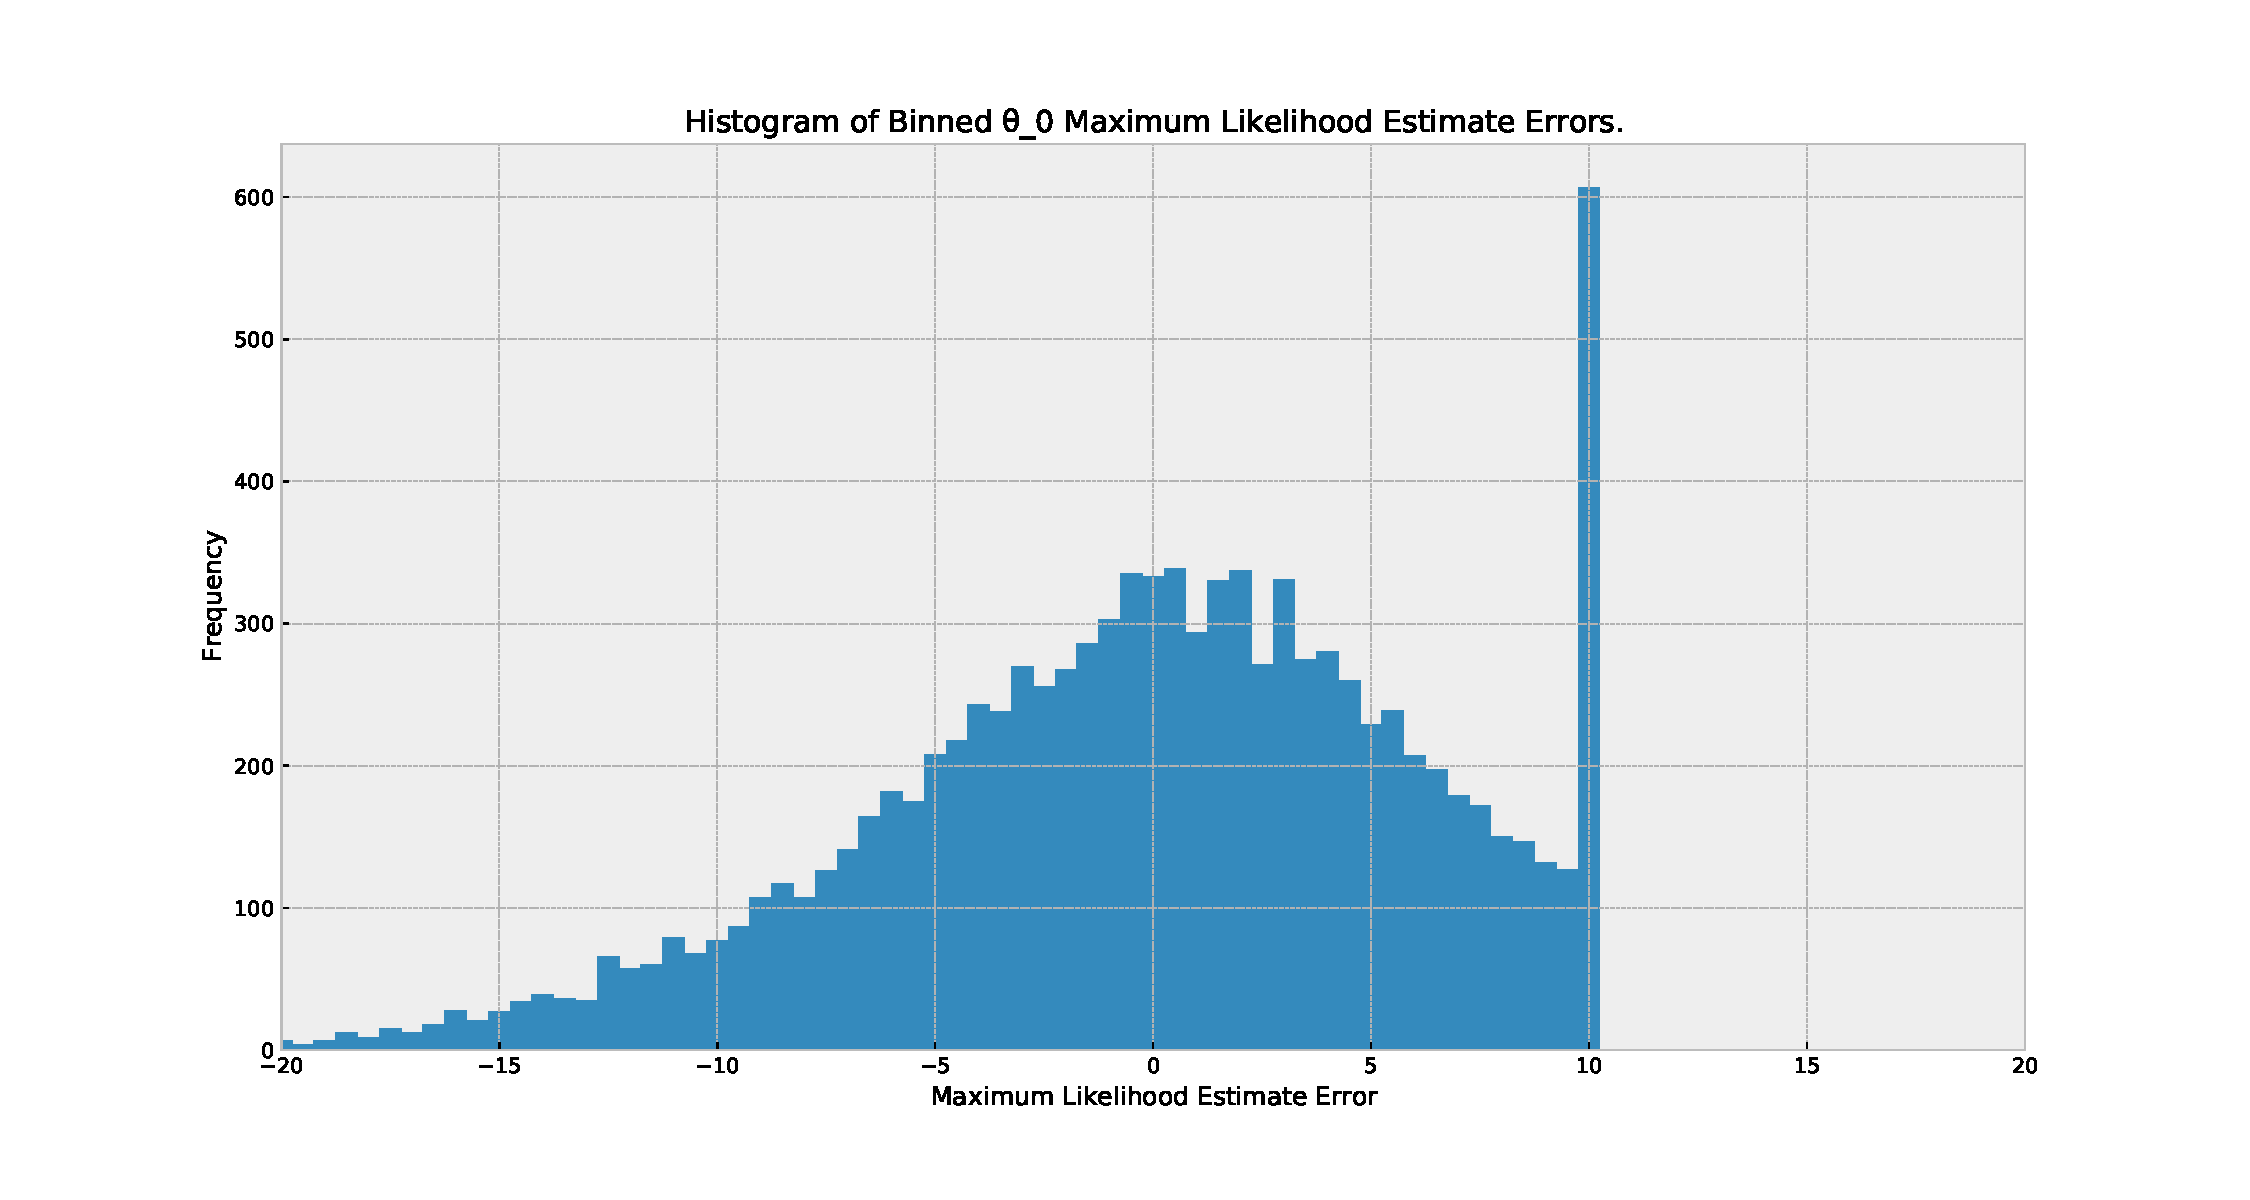
\includegraphics[height=10cm, width=16cm]{mle_error.pdf}
	\centering
	\caption{Histogram of Binned $\theta_0$ Maximum Likelihood Estimate Errors.}
	\label{fig:nhpp_mle_error}
\end{figure}
\\\\
The second approach we take is influenced by optimal design theory; an area in which experiments are designed with the aim of minimising the variance of estimators for statistical models. In \cite{optimum_design} and \cite{factorial_design}, the concept of D-optimality is presented. D-optimality, or `Determinant-optimality', is a criterion for evaluating an experimental design which states that the optimal design is the design whose information matrix has the greatest determinant.

In this context we will be using the Fisher Information matrix, and the intuition can be built for this by recalling the single parameter case. In the single parameter setting, the determinant is the value of the Fisher Information itself, which by its very nature is the value we wish to maximise. Recall that we compared the Fisher Information by taking the ratio of aggregated and raw cases, and so the parallel in the multi-parameter setting can be drawn. A naive extension of the metric for information loss in the multi-parameter setting is as follows:
\begin{equation}\label{eq:multi_info_loss}
	IL = 1 - \frac{\det \left( \mathcal{I}_{bin}(\theta) \right)}{\det \left( \mathcal{I}_{cts}(\theta) \right)}.
\end{equation}
Calculating this for our estimated Fisher Information matrices, we calculate an information loss in this setting of $IL=0.15$ by aggregating with $\Delta = 1/3$.

\section{Periodic Rate Function}\label{sec:trig_rate}
We now provide a derivation for an inhomogeneous Poisson process whose rate function is periodic, and we wish to perform inference on the rate parameter, $\omega$. We define our inhomogeneous Poisson process having rate function
\begin{equation}\label{eq:trig_rate}
	\lambda(t) = 1 + \cos(\omega t),
\end{equation}
and associated intensity function over interval $(a, b]$
\begin{equation}\label{eq:trig_intensity}
	\begin{aligned}
		\Lambda((a,b]) &= \int_a^b \lambda(t) \diff t = \int_a^b 1 + \cos(\omega t) \diff t \\
		&= (b - a) + \frac{1}{\omega} \left( \sin(\omega b) - \sin(\omega a) \right).
	\end{aligned}
\end{equation}

\subsection{Continuous Observations}
For continuous time observations, the log-likelihood function is of form:
\begin{equation}\label{eq:trig_log_likeli}
	\ell(\omega; t_1, t_2, ..., t_n) = \sum_{i=1}^n \log(1 + \cos(\omega t_i)) - ( T + \frac{1}{\omega} \sin(\omega T)).
\end{equation}
With Jacobian given by
\begin{equation*}
    \frac{\partial \ell}{\partial \omega} = - \sum_{i=1}^n \frac{t_i \sin(\omega t_i)}{\lambda(t_i)} - \frac{\omega T \cos(\omega T) - \sin(\omega T)}{\omega^2},
\end{equation*}
and Hessian
\begin{equation*}
		\frac{\partial^2 \ell}{\partial \omega^2} = -\sum_{i=1}^n \frac{t_i^2 \left(\cos(\omega t_i) + 1 \right)}{\lambda(t_i)^2}
		- \frac{(2 - \omega^2 T^2) \sin(\omega T) - 2 \omega T \cos(\omega T)}{\omega^3}.
\end{equation*}
\subsection{Aggregated Observations}
For binned-data with $K$ $\Delta$-width bins (with associated counts $n_0, n_1, ..., n_{K-1}$), the log-likelihood function is of form:
\begin{equation}\label{eq:trig_loglikeli_binned}
	\ell(x_0, x_1, x_2; n_0, ..., n_{K-1}) = \sum_{k=0}^{K-1} n_k \log( \Lambda(B_k) ) - \Lambda(T),
\end{equation}
where Mean measure over bin $B_k$ is given by 
\begin{equation}
	\Lambda(B_k) = \Delta + \frac{\sin((k+1) \Delta \omega) - \sin(k \Delta \omega)}{\omega}.
\end{equation}
The Jacobian and Hessian are of the forms

\begin{equation*}
	\begin{aligned}
		\frac{\partial \ell}{\partial \omega} &= \frac{\Delta}{\omega} \sum_{k=0}^{K-1} n_k \frac{
			(k+1) \cos \left( (k+1) \Delta \omega \right) - k \cos (k \Delta \omega)
		}{
			\Lambda(B_k)
		} \\
		&- \frac{1}{\omega^2} \sum_{k=0}^{K-1} n_k \frac{
			\sin \left((k+1) \Delta \omega \right) - \sin(k \Delta \omega)
		}{
			\Lambda(B_k)
		}\\
		&- \frac{1}{\omega^2} \left( \omega T \cos(\omega T) - \sin(\omega T) \right)
		,
	\end{aligned}
\end{equation*}
and
\begin{equation*}
	\begin{aligned}
		\frac{\partial^2 \ell}{\partial \omega^2} &= \frac{\Delta^2}{\omega} \sum_{k=0}^{K-1} n_k \frac{
			k^2 \sin \left(k \Delta \omega \right) - (k+1)^2 \sin \left((k+1) \Delta \omega \right)
		}{
			\Lambda(B_k)
		} \\
		&+ \frac{2}{\omega^3} \sum_{k=0}^{K-1} n_k \frac{
			\sin \left(\Delta (k+1) \omega \right) - \sin(\Delta k \omega)
		}{
			\Lambda(B_k)
		} \\
		&- \frac{2 \Delta}{\omega^2}\sum_{k=0}^{K-1} n_k \frac{
			(k+1) \cos \left(\Delta (k+1) \omega \right) - k \cos (\Delta k \omega)
		}{
			\Lambda(B_k)
		}\\
		&- \sum_{k=0}^{K-1} n_k \frac{
			\left(
				\frac{\Delta}{\omega} \left((k+1) \cos(\Delta (k+1) \omega) - k \cos(\Delta k \omega) \right)
				- \frac{1}{\omega^2} \left( sin(\Delta (k+1) \omega) - \sin (\Delta k \omega) \right)
			\right) ^ 2
		}{
			\Lambda(B_k) ^ 2
		} \\
		&- \frac{(2 - \omega^2 T^2) \sin(\omega T) - 2 \omega T \cos(\omega T)}{\omega^3}
		,
	\end{aligned}
\end{equation*}
respectively.
\subsection{Information Loss}
As discussed in Section \ref{sec:identifiability}, one of our focuses on the loss of information in this section will be model identifiability. Intuitively, if our bins are too large relative to the frequency of our rate function, we will not be able to correctly perform inference on it, as one or more of the peaks and troughs of the function will be captured within one bin. 

This topic of sampling frequency for periodic functions has been dealt with extensively in signal processing literature. A key definition in this area is the Nyquist rate. \\\\
Given a function with highest frequency $B$, the Nyquist rate \cite{nyquist} --- which is equal to $2B$ --- specifies the rate we must sample the function with to be free of the distortion known as aliasing. In this setting, our only periodic function is $\cos(\omega t)$, which has frequency $f = \omega / (2 \pi)$, meaning we also have that $B = \omega / (2 \pi)$; giving a Nyquist rate of $2B = \omega / \pi$.

This Nyquist rate gives an insight into how small our bins must be for us to be able to perform inference in this setting. If we set $\Delta < \omega / \pi$, we should be able to infer the value of $\omega$ with a reasonable degree of accuracy. If $\Delta$ is greater than this threshold, we could expect to see issues with model identifiability, as we do not have a high enough degree of resolution to observe changes in rate, as the periodicity will be lost within each bin.

This is, however, only a guideline. We find that even for values of $\Delta$ above this threshold, if $\Delta$ is not an integer factor of $\omega$, then inference is still possible (albeit with the requirement for an enormous increase in sample size). This is because the bins are moving in and out of phase with the intensity function, which eventually allow us to correctly infer the value of $\omega$. \\\\
We now perform inference for a toy problem with 3 different values of $\Delta$ to demonstrate the effect of binning on inference in this setting. We define our rate function:
\begin{equation*}
	\lambda(t) = 1 + \cos(\pi t),
\end{equation*}
with $T=25$. The Nyquist rate in this setting is $2B=1$. This defines our reasonable upper limit for $\Delta$. In order to have $\Delta=1$ with $T=25$, we would require $K=25$ bins; to avoid any potential boundary issues, we will choose our `threshold' value of $K$ to be $K=26$ bins, giving $\Delta=25/26$. To demonstrate over-aggregation, we will take half this value, with $K=13$, giving $\Delta=25/13$. Finally, to demonstrate a much safer level of aggregation, we will use $K = 50$ bins, giving $\Delta=0.5$. Figure \ref{fig:nhpp_periodic_unid} below shows an example simulation for $K=13$.
\begin{figure}[!h]
	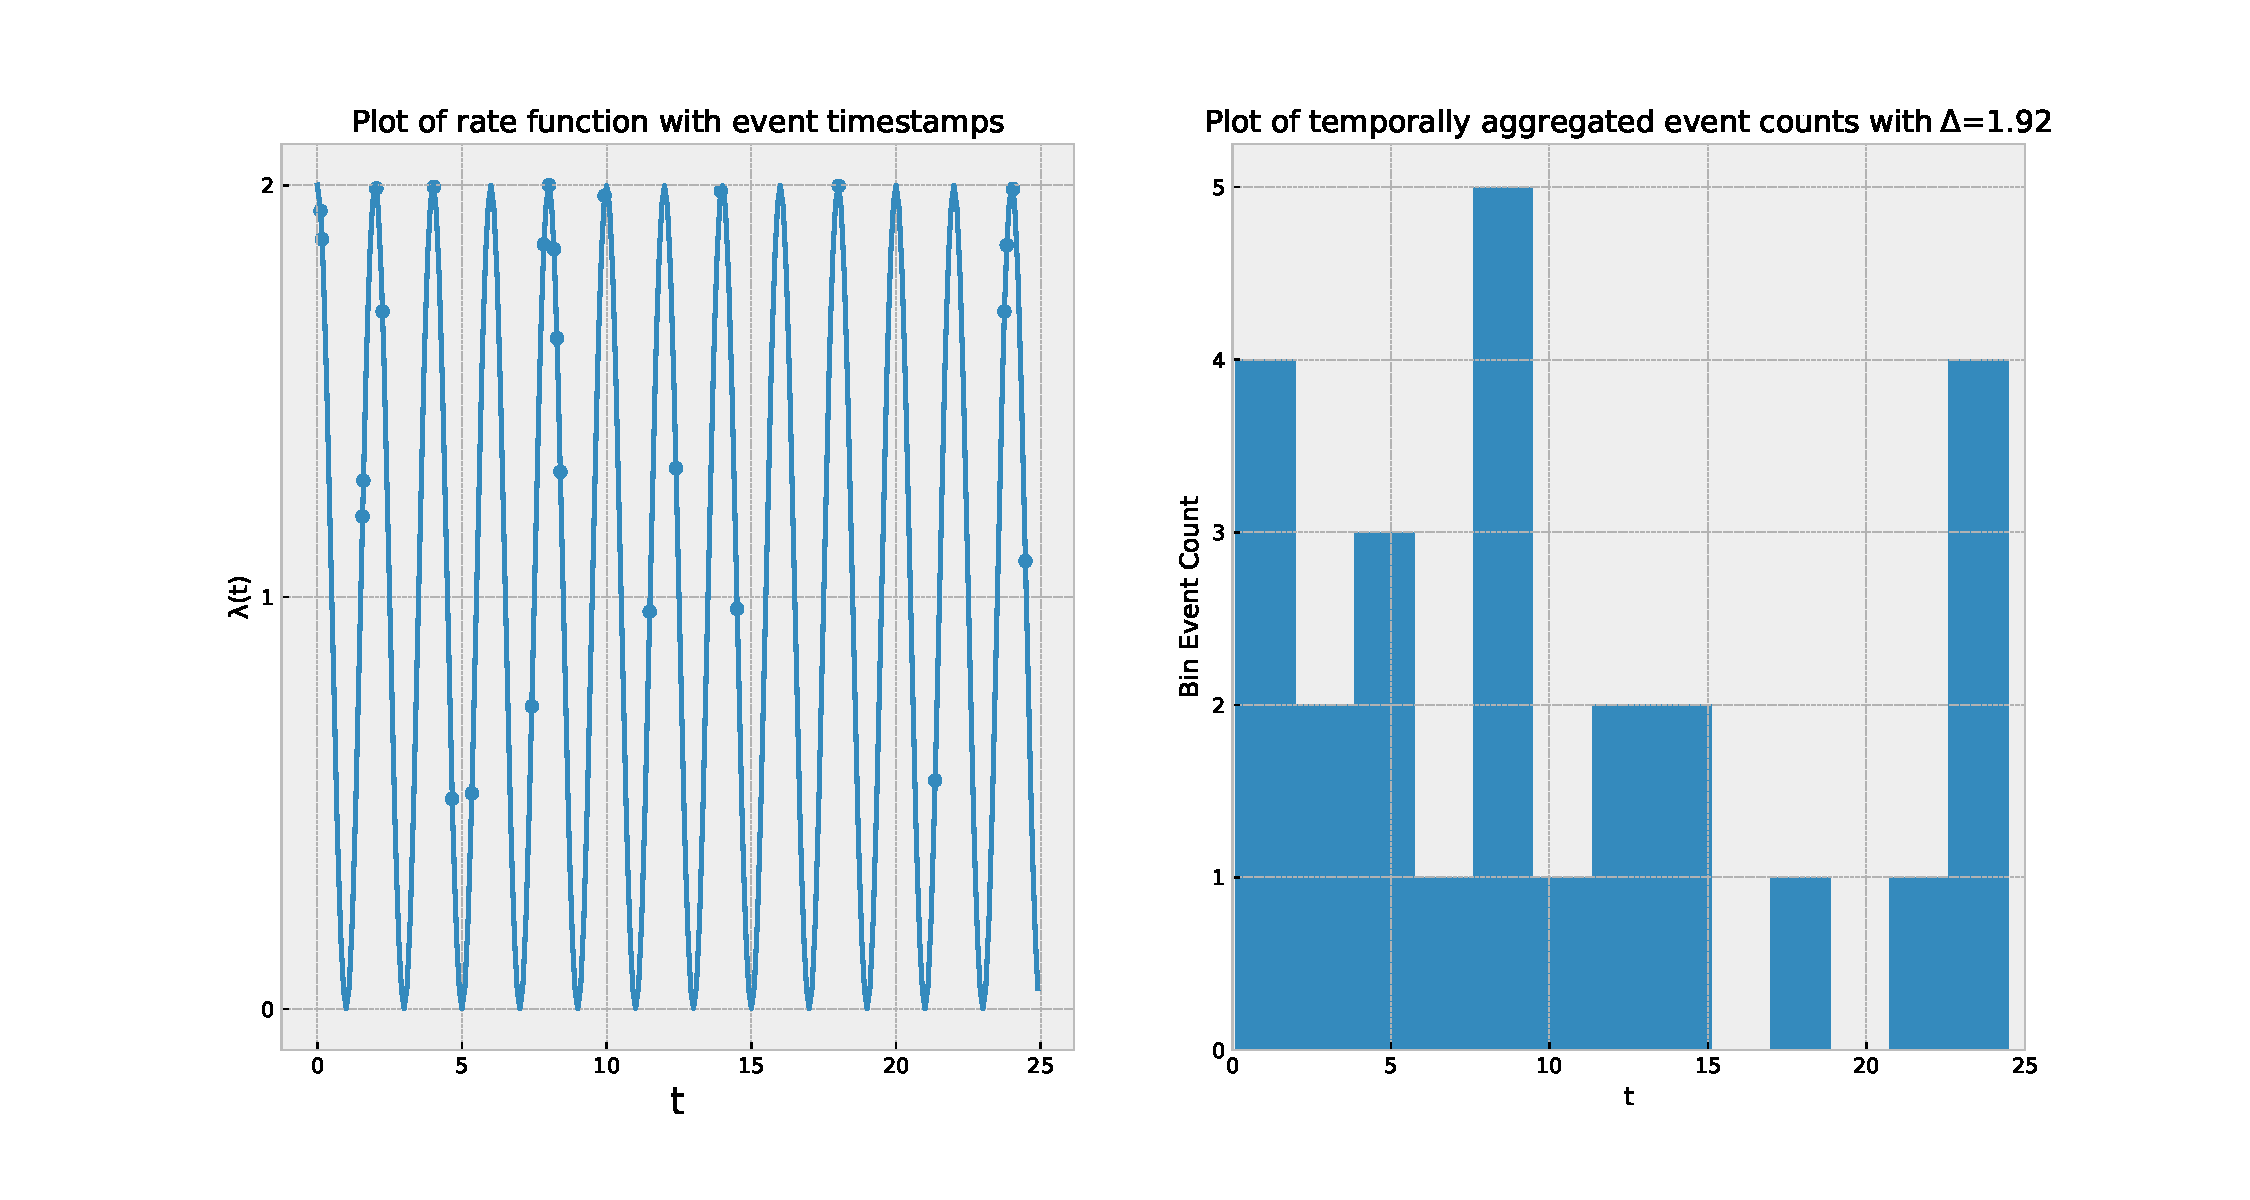
\includegraphics[height=10cm, width=16cm]{nhpp_periodic_unid.pdf}
	\centering
	\caption{Plots for inhomogeneous Poisson process with $\lambda(t)= 1 + \cos(\pi t)$.}
	\label{fig:nhpp_periodic_unid}
\end{figure}
\newpage\noindent
We begin in the `safe' aggregation setting, with $K=50$ and $\Delta=0.5$. Figure \ref{fig:nhpp_periodic_id_log_likeli} shows the log-likelihood curves for the raw and aggregated processes in one simulation of this setting. We can see from this figure that both approaches identify the true parameter $\omega = \pi$ almost exactly. Further, the maximum for the aggregated log-likelihood is clearly the only maximum in its region, with the function dropping away rapidly on both sides. There is no issue with model identifiability with this degree of resolution.
\begin{figure}[!h]
	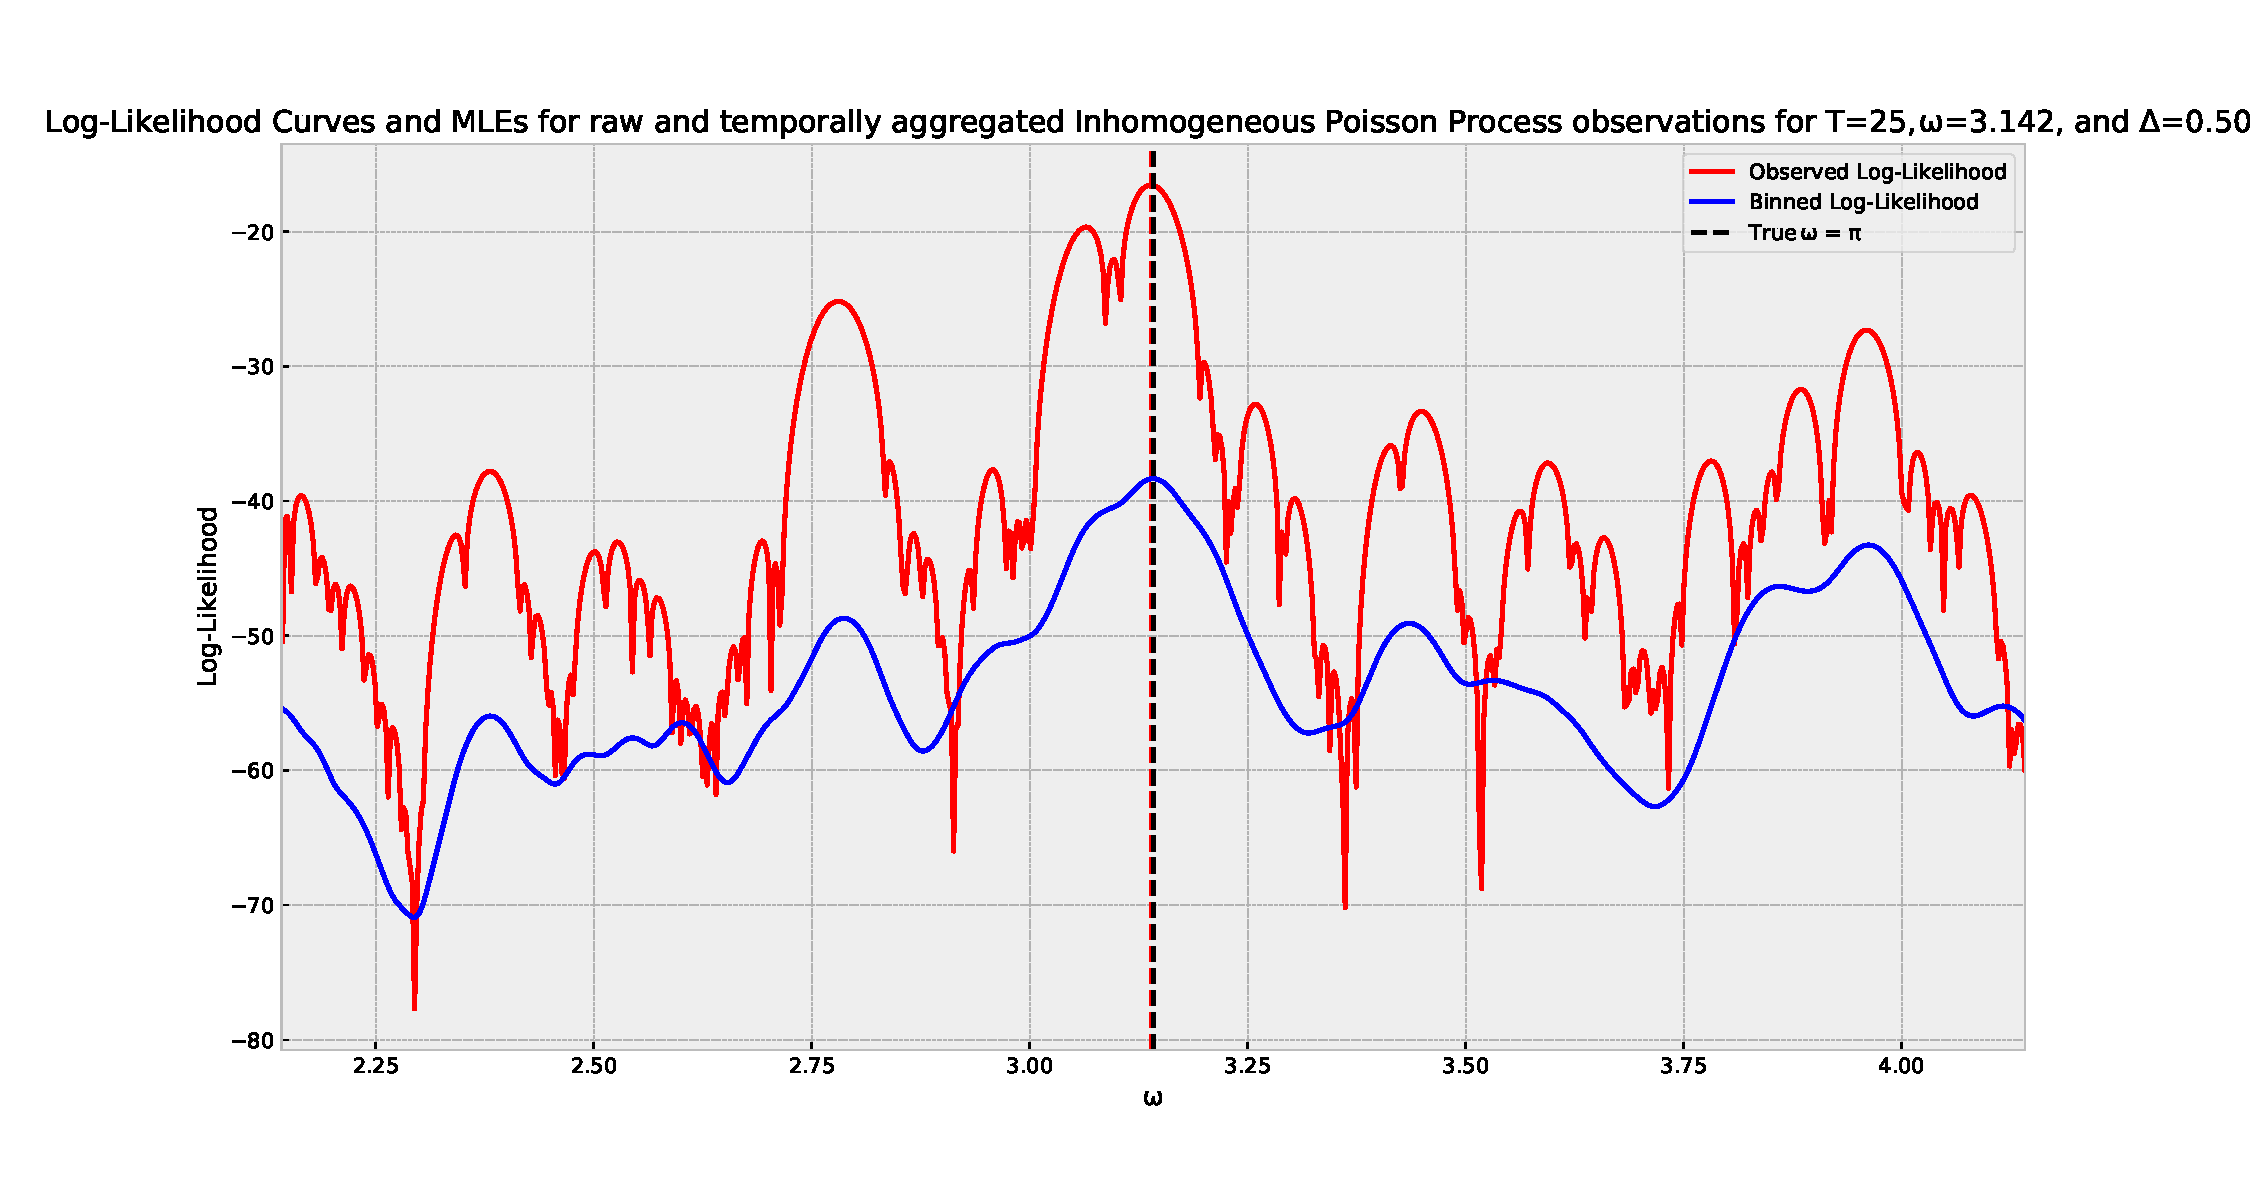
\includegraphics[height=10cm, width=16cm]{nhpp_periodic_id_log_likeli.pdf}
	\centering
	\caption{Observed log-likelihood curves for raw and aggregated inhomogeneous Poisson process observations with $\lambda(t)= 1 + \cos(\pi t), \Delta=0.5$.}
	\label{fig:nhpp_periodic_id_log_likeli}
\end{figure}
\newpage\noindent
Figure \ref{fig:nhpp_periodic_unid_log_likeli}, however, shows a different story. In this, we are showing a simulation in the setting where $K=13$, and $\Delta=25/13$. While the raw observations' log-likelihood function again estimates the value of $\omega=\pi$ almost exactly; the maximum likelihood estimate in the binned case is much further away, with $\hat{\omega}_{bin} = 4.094$. Further, we can see that the binned log-likelihood curve is almost completely flat over the plotted range. This is a clear demonstration of practical identifiability for this model: the flatness of the curve demonstrates a Hessian with value near 0, meaning the Information matrix is, very nearly, non-invertible. It is impossible to perform inference in a setting such as this where we have over-aggregated our data; the periodicity has been lost in the bins.
\begin{figure}[!h]
	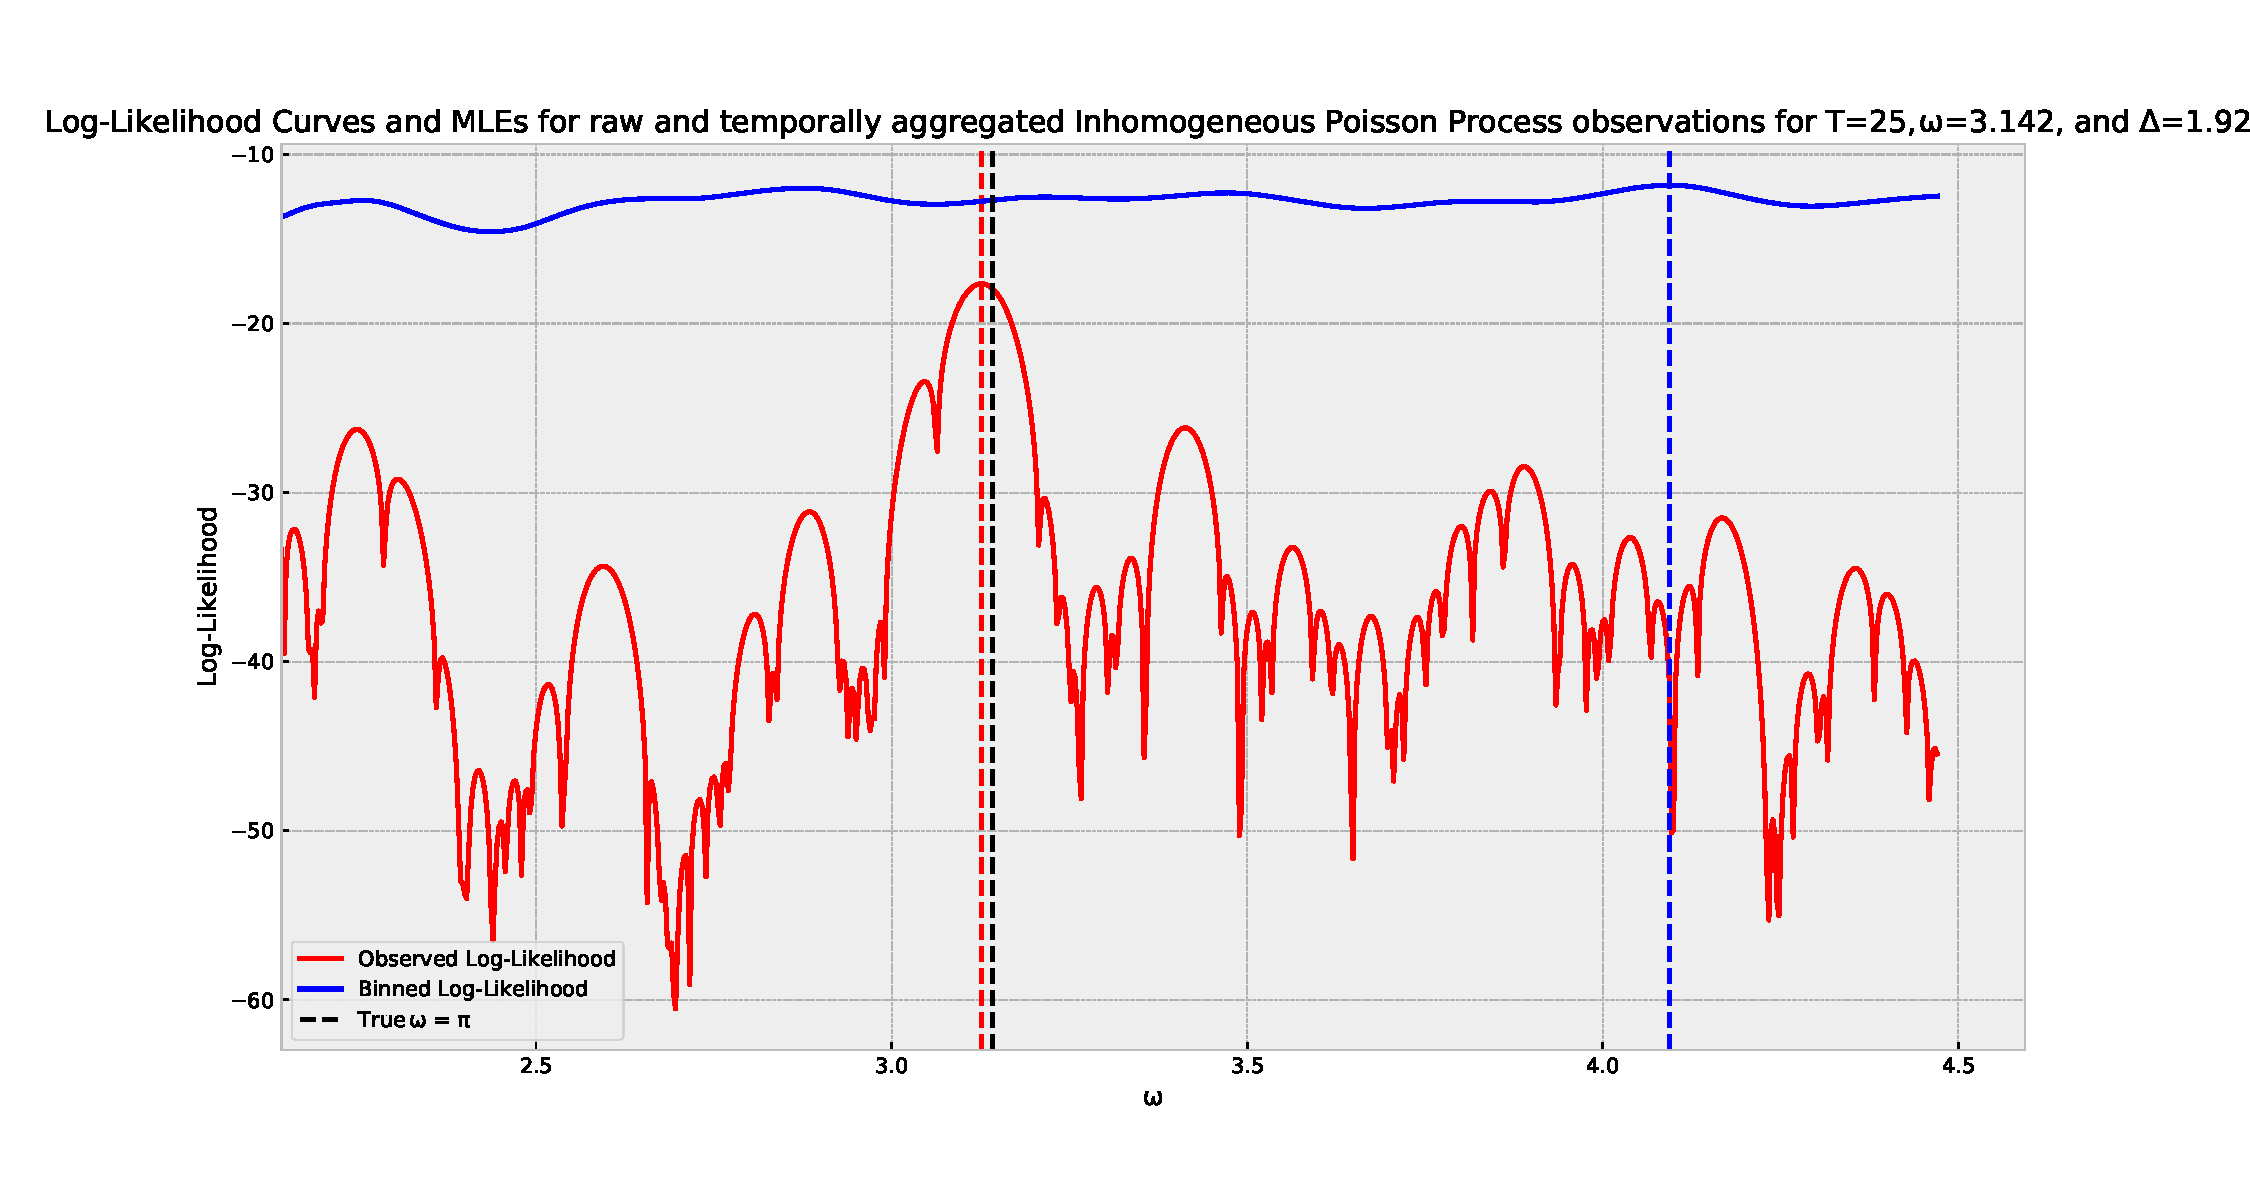
\includegraphics[height=10cm, width=16cm]{nhpp_periodic_unid_log_likeli.pdf}
	\centering
	\caption{Observed log-likelihood curves for raw and aggregated inhomogeneous Poisson process observations with $\lambda(t)= 1 + \cos(\pi t), \Delta=25/13$. Demonstrating practical unidentifiability due to over-aggregation.}
	\label{fig:nhpp_periodic_unid_log_likeli}
\end{figure}
\newpage\noindent
We conclude this section by estimating the Fisher Information (via Monte Carlo estimation with 1000 simulations) for $\omega$ given the three levels of aggregation above, along with showing maximum likelihood estimate errors in each case. Table \ref{tab:nhpp_periodic_errors} shows these results below. As usual, we can see that as the aggregation increases, the estimated Fisher Information decreases, and our estimates become more variable as a result.
\begin{table}[ht]
	\centering
	\begin{tabular}{|c|c|c|c|c|}
	\hline
		$\hat{\omega}$ & Mean Error & Std Dev & Estimated Fisher Info & Info Loss \\
	\hline
		Continuous & 0.0083 & 0.1148 & 4413.7265 & 0 \\
	\hline
		$\Delta=0.5$  & 0.0159 & 0.2781 & 3292.7933 & 0.2540 \\
	\hline
		$\Delta=25/26$  & 0.0553 & 0.4262 & 1635.2861 & 0.6295 \\
	\hline
		$\Delta=25/13$  & 0.5076 & 0.8560 & 681.7895 & 0.8472 \\
	\hline
	\end{tabular}
	\caption{Table showing maximum likelihood estimate statistics of periodic rate parameter $\omega$ in continuous and three aggregated settings, with $\omega=\pi, T=25$.}
	\label{tab:nhpp_periodic_errors}
\end{table}\\
Focusing once more on $\Delta=25/13$, at first glance it may appear that the mean error is not so bad, that the variability is reasonable. However this masks a larger issue that has occurred in the over-aggregated setting. The maximum likelihood estimates are very rarely near the true parameter. Figure \ref{fig:overaggregated_error_kde} shows the kernel density estimate for the error distribution of our maximum likelihood estimate. We can see from this that the model truly is unidentifiable at this level of aggregation, as there are two clusters of incorrect estimates: one cluster greater than the true value, and one cluster less than it.
\begin{figure}[!h]
	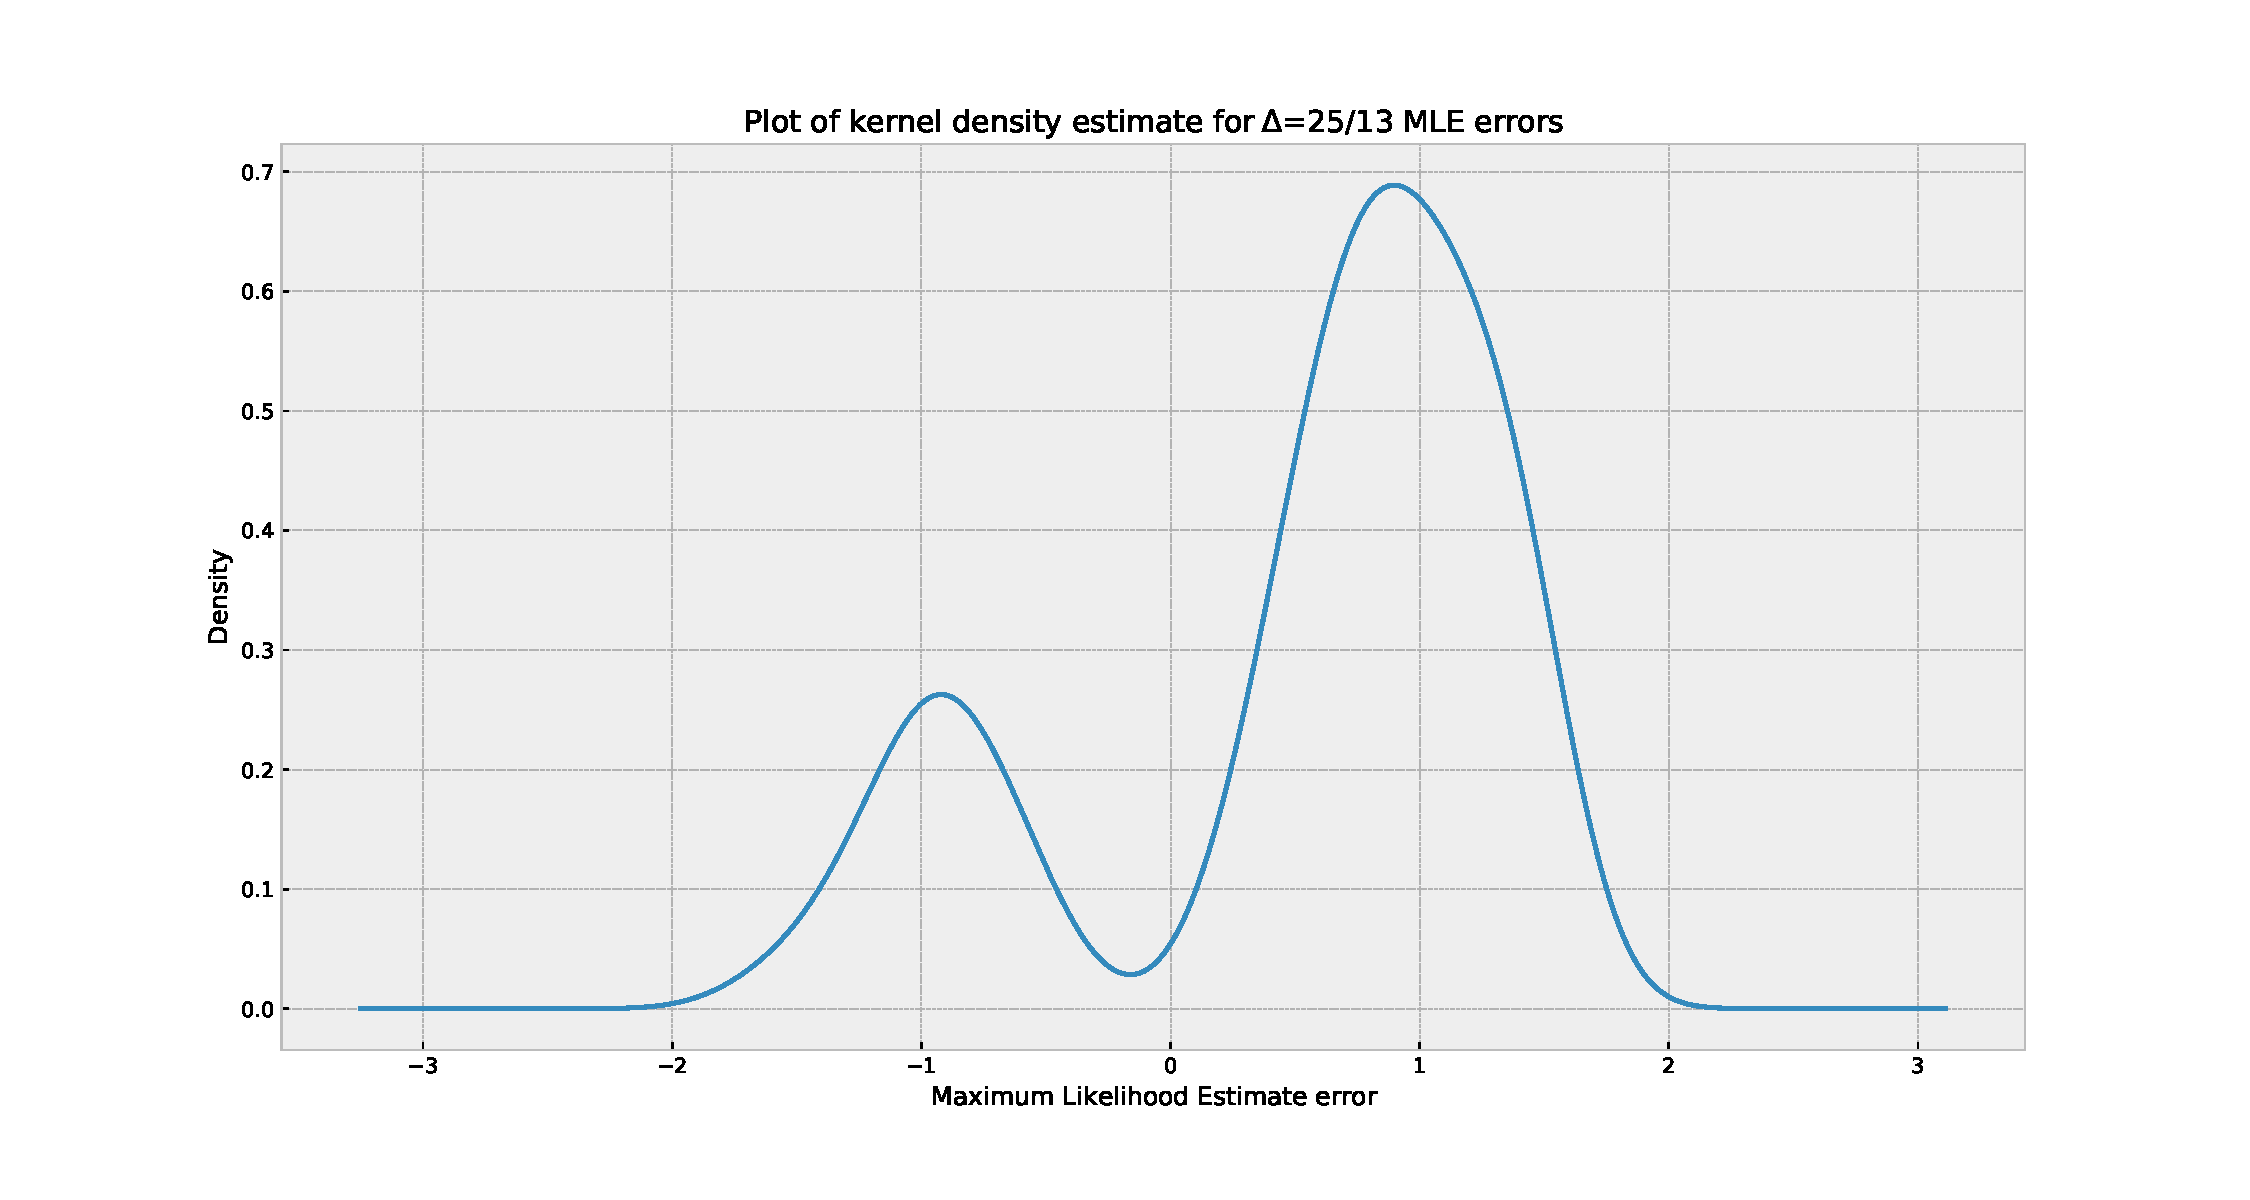
\includegraphics[height=7.5cm, width=14cm]{overaggregated_error_kde.pdf}
	\centering
	\caption{Plot of kernel density estimate for maximum likelihood estimate errors with $T=25,K=13,\Delta=25/13$.}
	\label{fig:overaggregated_error_kde}
\end{figure}
\chapter{Another Approach - Uniform Resampling}\label{chapter:resampling}
The results derived so far have broadly taken the same approach: calculate the log-likelihood for the aggregated observations; take first and second derivatives with respect to the parameters of interest; and analytically or numerically calculate the Fisher information from this.

While this approach works for simpler problems, for more complicated examples --- for example, performing inference on aggregated data for Hawkes processes --- the binned log-likelihood may be analytically intractable. For these instances, an approach used in \cite{uniform_resampling} provides an alternative.

Say we are given the bins $B_k$ and associated counts $n_k$ for some inference problem for which we have the continuous-form log-likelihood. Instead of trying to evaluate the binned log-likelihood directly, we can uniformly sample $n_k$ `reconstructed' observations for bin $B_k$ and treat these as if they were our raw observations. In this way, we make no strong \emph{a priori} assumptions on the structure of our data.

We will perform this on one of the previously explored inference problems, the univariate normal, in order to evaluate its performance relative to the derived binned log-likelihood approach.

\section{Univariate Normal}
We return to the univariate Normal distribution, with density function as given in \ref{eq:normal_pdf}. In order to evaluate the relative performance of the three approaches --- raw, continuous data; binned data with log-likelihood approach; and binned data with uniform resampling --- we will run simulations for different bin size, sample size and parameter configurations. For all configurations we run 1000 iterations of 500 Normally distributed observations. We examine the mean and standard distribution of the three approaches' maximum likelihood estimates in all cases. Before this, we also note that all methods estimated had negligible average error for their $\mu$ estimates, these tables \ref{tab:mu_hat_error}, \ref{tab:mu_hat_error_offset} are shown in the Appendix.
\newpage\noindent
We will first examine inference performed on various zero-mean Normal distributions:\\\\
Table \ref{tab:mu_hat_std} shows the standard deviations of the error between the true value $\sigma$ and maximum likelihood estimates $\hat{\sigma}, \hat{\sigma}_{bin}, $ and $\hat{\sigma}_{resample}$. We can see that for the first two cases, as the binning increases, our estimates for $\mu$ become more variable. This is more pronounced in the uniformly resampled approach, with a $20\%$ increase in standard deviation as $\Delta$ goes from 1 to 2.

Another point of interest from this table is by comparing the first and third rows. The difference here is $\sigma=1$ vs $\sigma=2$. We can see that the relative increase in standard deviation is lower, again reinforcing the points made in Section \ref{subsec:normal_info_loss}.
\begin{table}[ht]
	\centering
	\begin{tabular}{|c|c|c|c|}
	\hline
	Parameters & $\mu - \hat{\mu}$ Std Dev & $\mu - \hat{\mu}_{bin}$ Std Dev & $\mu - \hat{\mu}_{resample}$ Std Dev \\
	\hline
		$\mu=0, \sigma=1, \Delta=1$ & $0.0466$ & $0.0486$ & $0.0504$ \\
	\hline
		$\mu=0, \sigma=1, \Delta=2$ & $0.0454$ & $0.0528$ & $0.0608$ \\
	\hline
		$\mu=0, \sigma=2, \Delta=1$ & $0.0901$ & $0.0910$ & $0.9272$ \\
	\hline
	\end{tabular}
	\caption{Table showing three data-scenario standard deviation in $\mu$ maximum likelihood estimate errors for three zero-mean normal inference problems.}
	\label{tab:mu_hat_std}
\end{table}\\\noindent
Tables \ref{tab:sigma_hat_mean} and \ref{tab:sigma_hat_std} show the means and standard deviations in maximum likelihood estimate errors for $\sigma$, respectively, for the three same inference problems. As we are using the unadjusted maximum likelihood estimate, there will be a bias on the order of $\frac{n}{n-1} \approx 0.2\%$ for $n=500$ in the continuous setting. In the first two rows, we can see the effect of increased aggregation in the resampled case. It has a pronounced bias in over-estimating the value of $\sigma$, even for a large sample size, and this bias increases as $\Delta$ increases.

Again, as $\sigma$ itself increases relative to $\Delta$, the relative bias decreases. This is due to the aggregation having less of an effect as the observations themselves will be more spread out.
\begin{table}[ht]
	\centering
	\begin{tabular}{|c|c|c|c|}
	\hline
		Parameters & $\sigma - \hat{\sigma}$ Mean & $\sigma - \hat{\sigma}_{bin}$ Mean & $\sigma - \hat{\sigma}_{resample}$ Mean  \\
	\hline
		$\mu=0, \sigma=1, \Delta=1$ & $0.0007$ & $0.0007$ & $-0.0800$ \\
	\hline
		$\mu=0, \sigma=1, \Delta=2$ & $0.0011$ & $0.0042$ & $-0.3009$ \\
	\hline
		$\mu=0, \sigma=2, \Delta=1$ & $0.0010$ & $0.0006$ & $-0.0407$ \\
	\hline
	\end{tabular}
	\caption{Table showing three data-scenario average $\sigma$ maximum likelihood estimate errors for three zero-mean Normal inference problems.}
	\label{tab:sigma_hat_mean}
\end{table}
\begin{table}[ht]
	\centering
	\begin{tabular}{|c|c|c|c|}
	\hline
	Parameters & $\sigma - \hat{\sigma}$ Std Dev & $\sigma - \hat{\sigma}_{bin}$ Std Dev & $\sigma - \hat{\sigma}_{resample}$ Std Dev \\
	\hline
		$\mu=0, \sigma=1, \Delta=1$ & $0.0312$ & $0.0340$ & $0.0345$ \\
	\hline
		$\mu=0, \sigma=1, \Delta=2$ & $0.0309$ & $0.0417$ & $0.0364$ \\
	\hline
		$\mu=0, \sigma=2, \Delta=1$ & $0.0635$ & $0.0647$ & $0.0642$ \\
	\hline
	\end{tabular}
	\caption{Table showing three data-scenario standard deviation in $\sigma$ maximum likelihood estimate errors for three zero-mean Normal inference problems.}
	\label{tab:sigma_hat_std}
\end{table}
\newpage\noindent
We now explore how the three approaches compare in the case where $\mu \neq 0$. The motivation for this is discussed in Section \ref{subsec:normal_info_loss}, where our ability to perform inference in the binned setting is partially dependent on whether bin edges align with $\mu$.

Tables \ref{tab:sigma_hat_mean_offset} and \ref{tab:sigma_hat_std_offset} show the means and standard deviations in maximum likelihood estimate errors between the true value $\mu$ and maximum likelihood estimates $\hat{\sigma}, \hat{\sigma}_{bin}, $ and $\hat{\sigma}_{resample}$. Again, we can see that increased binning quickly leads to a biased estimate in the uniformly resampled case. We also see again that increased binning results in greater variability in our estimates for both the binned and resampled cases. \\\\
One final point to note here is the case where $\Delta=0.05$. The difference in our ability to perform inference at this low level of aggregation is almost negligible for this inference problem. The errors in estimation are very similar, both in their average value, and their variability. In fact, at 4 decimal places of precision, the standard deviation in the errors is identical for all three approaches.

\begin{table}[ht]
	\centering
	\begin{tabular}{|c|c|c|c|}
	\hline
		Parameters & $\sigma - \hat{\sigma}$ Mean & $\sigma - \hat{\sigma}_{bin}$ Mean & $\sigma - \hat{\sigma}_{resample}$ Mean  \\
	\hline
		$\mu=0.5, \sigma=1, \Delta=1$ & $0.0012$ & $0.0015$ & $-0.0784$ \\
	\hline
		$\mu=0.5, \sigma=1, \Delta=2$ & $0.0019$ & $0.0043$ & $-0.2875$ \\
	\hline
		$\mu=0.5, \sigma=1, \Delta=0.05$ & $0.0030$ & $0.0030$ & $0.0028$ \\
	\hline
	\end{tabular}
	\caption{Table showing three data-scenario average $\sigma$ maximum likelihood estimate errors for three non-zero-mean Normal inference problems.}
	\label{tab:sigma_hat_mean_offset}
\end{table}
\begin{table}[ht]
	\centering
	\begin{tabular}{|c|c|c|c|}
	\hline
	Parameters & $\sigma - \hat{\sigma}$ Std Dev & $\sigma - \hat{\sigma}_{bin}$ Std Dev & $\sigma - \hat{\sigma}_{resample}$ Std Dev \\
	\hline
		$\mu=0.5, \sigma=1, \Delta=1$ & $0.0320$ & $0.0345$ & $0.0342$ \\
	\hline
		$\mu=0.5, \sigma=1, \Delta=2$ & $0.0318$ & $0.0421$ & $0.0408$ \\
	\hline
		$\mu=0.5, \sigma=1, \Delta=0.05$ & $0.0321$ & $0.0321$ & $0.0321$ \\
	\hline
	\end{tabular}
	\caption{Table showing three data-scenario standard deviation in $\sigma$ maximum likelihood estimate errors for three non-zero-mean Normal inference problems.}
	\label{tab:sigma_hat_std_offset}
\end{table}

\chapter{Conclusion}
In this thesis we have explored the effect data aggregation has on our ability to perform statistical inference in multiple settings. In order to do this we have calculated log-likelihood forms for aggregated inference problems, and used these to find the Fisher Information for parameters of interest.

By doing so we have been able to quantify a loss in the resolution of inference dependent on both the problem at hand, and the degree of aggregation being applied. \\\\
This work may naturally be extended to many other inference problems. For inference on distributions, an extension to multivariate Normal distributions with non-zero off-diagonal covariance matrix values would likely be a fruitful topic to explore; along with extending the work to any other standard distributions.

The nature of the inference problems we investigated in the distribution setting mostly allowed for us to simply compare parameter-wise Fisher Information, due to the problems being either one-dimensional, or the Fisher Information matrices being diagonal. We explored one approach for quantifying information loss in multi-parameter inference problems where the Fisher Information matrix was not diagonal: by comparing the determinant of the Fisher Information matrices. This is an area which could benefit from further exploration, or even alternative approaches (such as using the trace of the Fisher Information matrix). \\\\
For stochastic processes, we have only scratched the surface. Our approach on Poisson processes has demonstrated a general technique which can be applied to most common rate function forms. However, as discussed in Chapter \ref{chapter:resampling}, there are many other forms of stochastic processes which we may want to perform inference on whose binned log-likelihoods are intractable. The approach we have demonstrated here could be applied to other stochastic processes to examine the effect of data aggregation on inference for those.


\cleardoublepage
\phantomsection
\addcontentsline{toc}{chapter}{\bibname} % Add an entry for the Bibliography in the Table of Contents
%\pagestyle{headings}
\bibliographystyle{abbrvnat} % set the bibliography style
\bibliography{bibtexfile} % generate the bibliography
% Pick a sensible bibliography style. 
% If like above you choose to use author-year style citations, you must choose a natbib-compatible bibliographystyle such as 'plainnat'. Abbrvnat is one of the few built-in styles of this type. You may find many more bibliography styles (*.bst files) online. You can also choose to write your bibliography manually instead of using BibTeX (This will take you longer, unless you plan to use the content of a BibTeX-generated *.bbl file as your starting point).
% When creating a BibTeX file using e.g. reference manager software, note that the entries may contain additional unwanted fields which you would then need to erase. For example, you probably don't want to include the URL of a journal paper in your bibliography.


%\cleardoublepage \fancyhead[L]{APPENDIX}
\appendix % This line declares that you are starting the appendix.
% If you want a single Appendix and want it to be called Appendix instead of Appendix A, the following should work:
%\setcounter{secnuk Depth}{-1} %This turns off automatic chapter numbering

\chapter{Code}
All code can be found in the GitHub repository \href{https://github.com/Tom-Crow/thesis}{Thesis}.
\begingroup
\let\clearpage\relax
\chapter{Tables}
\begin{table}[ht]
	\centering
	\begin{tabular}{|c|c|c|}
	\hline
		Parameter & MLE Mean Error & MLE$_{bin}$ Mean Error \\
	\hline
		$\theta_0$ & $-0.0032$ & $-0.0136$ \\
	\hline
		$\theta_1$  & $0.0248$ & $0.0271$ \\
	\hline
		$\theta_2$  & $0.0006$ & $0.0467$ \\
	\hline
		$\theta_3$  & $-0.00003$ & $0.0011$ \\
	\hline
	\end{tabular}
	\caption{Table showing mean errors for maximum likelihood estimates of polynomial rate parameters in continuous and aggregated setting. Rate function is of form $\lambda(t) = \theta_0 + \theta_1 t + \theta_2 t^2 + \theta_3 t^3.$}
	\label{tab:nhpp_poly_err}
\end{table}

\begin{table}[ht]
	\centering
	\begin{tabular}{|c|c|c|c|}
	\hline
		Parameters & $\mu - \hat{\mu}$ Mean & $\mu - \hat{\mu}_{bin}$ Mean & $\mu - \hat{\mu}_{resample}$ Mean  \\
	\hline
		$\mu=0, \sigma=1, \Delta=1$ & $0.0009$ & $0.0015$ & $0.0017$ \\
	\hline
		$\mu=0, \sigma=1, \Delta=2$ & $0.0006$ & $0.0004$ & $-0.0002$ \\
	\hline
		$\mu=0, \sigma=2, \Delta=1$ & $-0.0001$ & $-0.0005$ & $-0.0008$ \\
	\hline
	\end{tabular}
	\caption{Table showing three data-scenario average $\mu$ maximum likelihood estimate errors for three zero-mean Normal inference problems.}
	\label{tab:mu_hat_error}
\end{table}
\begin{table}[ht]
	\centering
	\begin{tabular}{|c|c|c|c|}
	\hline
		Parameters & $\mu - \hat{\mu}$ Mean & $\mu - \hat{\mu}_{bin}$ Mean & $\mu - \hat{\mu}_{resample}$ Mean  \\
	\hline
		$\mu=0.5, \sigma=1, \Delta=1$ & $-0.0009$ & $-0.0009$ & $-0.0012$ \\
	\hline
		$\mu=0.5, \sigma=1, \Delta=2$ & $0.0014$ & $0.0012$ & $-0.0019$ \\
	\hline
		$\mu=0.5, \sigma=1, \Delta=0.05$ & $-0.0007$ & $-0.0007$ & $-0.0007$ \\
	\hline
	\end{tabular}
	\caption{Table showing three data-scenario average $\mu$ maximum likelihood estimate errors for three non-zero-mean Normal inference problems.}
	\label{tab:mu_hat_error_offset}
\end{table}
\begin{table}[ht]
	\centering
	\begin{tabular}{|c|c|c|c|}
	\hline
	Parameters & $\mu - \hat{\mu}$ Std Dev & $\mu - \hat{\mu}_{bin}$ Std Dev & $\mu - \hat{\mu}_{resample}$ Std Dev \\
	\hline
		$\mu=0.5, \sigma=1, \Delta=1$ & $0.0435$ & $0.0455$ & $0.0472$ \\
	\hline
		$\mu=0.5, \sigma=1, \Delta=2$ & $0.0443$ & $0.0506$ & $0.0562$ \\
	\hline
		$\mu=0.5, \sigma=1, \Delta=0.05$ & $0.0448$ & $0.0447$ & $0.0447$ \\
	\hline
	\end{tabular}
	\caption{Table showing three data-scenario standard deviation in $\mu$ maximum likelihood estimate errors for three zero-mean Normal inference problems.}
	\label{tab:mu_hat_std_offset}
\end{table}
\endgroup
\end{document}